\documentclass[letterpaper, 10 pt, journal, twoside]{IEEEtran}
\usepackage{amsmath,amsfonts}
\usepackage{algorithmic}
\usepackage{algorithm}
\usepackage{array}
%\usepackage{subcaption}
\usepackage{textcomp}
\usepackage{stfloats}
\usepackage{url}
\usepackage{verbatim}
\usepackage{booktabs}
\usepackage{tabularx}



\usepackage{graphicx}
\usepackage{cite}
\hyphenation{op-tical net-works semi-conduc-tor IEEE-Xplore}
% updated with editorial comments 8/9/2021
\setlength{\abovedisplayskip}{3pt}
\setlength{\belowdisplayskip}{3pt}
\setlength{\abovedisplayshortskip}{2pt}
\setlength{\belowdisplayshortskip}{2pt}

\begin{document}
\bstctlcite{IEEEexample:BSTcontrol} 

\title{Humanoid Footstep Planning using Graphs of Convex Sets}

\author{Hyunseok Kim$^{1}$,
George Mesesan$^{2}$,~\IEEEmembership{Member,~IEEE},
Robert Schuller$^{2,3}$,
Jinoh Lee$^{1,2,\dagger}$,~\IEEEmembership{Senior Member,~IEEE},
and Hae-Won Park$^{1,\dagger}$,~\IEEEmembership{Member,~IEEE}%
\thanks{Manuscript received: May 12, 2026;
Revised: August 2, 2026;
Accepted: October 6, 2026.}%
\thanks{This paper was recommended for publication by Editor
Soon-Jo Chung upon evaluation of the Associate Editor and
Reviewers' comments.}%
\thanks{This work was supported in part by the Technology
Innovation Program (or Industrial Strategic Technology
Development Program-Robot Industry Technology Development)
under Grant RS-2024-00427719 (Dexterous and Agile Humanoid
Robots for Industrial Applications), funded by the Ministry
of Trade Industry \& Energy (MOTIE, Korea), and in part by
the National Research Council of Science \& Technology(NST)
grant by the Korea government (MSIT) (No. GTL25042-000).}%
\thanks{$^{1}$Authors are with the Department of Mechanical
Engineering, Korea Advanced Institute of Science and Technology,
Yuseong-gu, Daejeon 34141, Republic of Korea.
{\tt\footnotesize haewonpark@kaist.ac.kr}}%
\thanks{$^{2}$Authors are with the Institute of Robotics
and Mechatronics, German Aerospace Center (DLR),
Wessling, Germany.
{\tt\footnotesize Jinoh.Lee@dlr.de}}%
\thanks{$^{3}$The author is with the School of
Computation, Information and Technology,
Technical University of Munich (TUM),
85748 Garching, Germany.
}%
\thanks{$^{\dagger}$Co-corresponding authors.}%
\thanks{Digital Object Identifier (DOI): see top of this page.}%
}

\markboth{IEEE Robotics and Automation Letters. Preprint Version. Accepted October, 2026}
{Kim \MakeLowercase{\textit{et al.}}: Humanoid Footstep Planning using Graphs of Convex Sets}

\maketitle

\begin{abstract}
Footstep planning for humanoid robots requires simultaneously reasoning over discrete stepping sequences and continuous foot placements under strict time budgets. 
In this paper, we propose a graph-based optimization approach for humanoid footstep planning within the Graphs of Convex Sets (GCS) framework. 
We first formulate a nonconvex quadratically constrained quadratic program (QCQP) that captures terrain feasibility and kinematic reachability.
We then construct a mode-aware graph, where each node represents a kinematically feasible convex region associated with a locomotion mode and each edge encodes a feasible transition. 
By integrating the QCQP formulation with the graph structure, we cast the planning problem within the GCS framework and apply semidefinite programming to obtain a convex relaxation that does not require an initial discrete path or initial values for the continuous variables.
We validate the proposed planner through real-world deployment on the torque-controlled humanoid robot in a rhythm-based stepping scenario, where footsteps must be planned within strict timing constraints.
These results show that the method can compute high-quality footstep plans within real-time budgets, enabling reliable execution and validation on humanoid hardware.
\end{abstract}

\begin{IEEEkeywords}
Motion and Path Planning,
Humanoid and Bipedal Locomotion,
Optimization and Optimal Control
\end{IEEEkeywords}

\section{Introduction}
\IEEEPARstart{H}{umanoid} robots have high degrees of freedom (DOFs) enabling flexible and mobile behaviors \cite{Park2012finite,Jeong2019Robust,Lee2016Robust}, allowing them to traverse stairs, narrow passages, and cluttered spaces by stepping over or around obstacles.
However, generating feasible motions and safe footholds remains challenging, requiring environment-aware planning.
To address these mobility challenges, a variety of approaches have been explored. 
Recent learning-based locomotion policies have achieved robust traversal over challenging terrain, often without relying on explicit footstep planning\cite{zhang2026focusnav,kim2025high,yoon2025state,ben2025gallant,he2025attention}.
However, tasks involving sparse or constrained support regions still require accurate foot placement and efficient path selection to reach a specific goal.
Some studies therefore employ hierarchical planning frameworks \cite{calvert2022fast,mishra2024efficient}, where a global body path is first generated and refined through local footstep planning.
Meanwhile, footstep planners \cite{kuffner2001footstep,griffin2019footstep} explicitly reason about terrain geometry and kinematic feasibility to determine precise footholds.
One of the key challenges is to simultaneously handle the discrete problem of selecting a contact surface for each step and the continuous problem of determining the exact position and orientation of the foot on the respective surface. 
Among these, our work focuses on a footstep planner that directly tackles both the discrete and continuous aspects of the problem.

\begin{figure}[t]
    \centering
    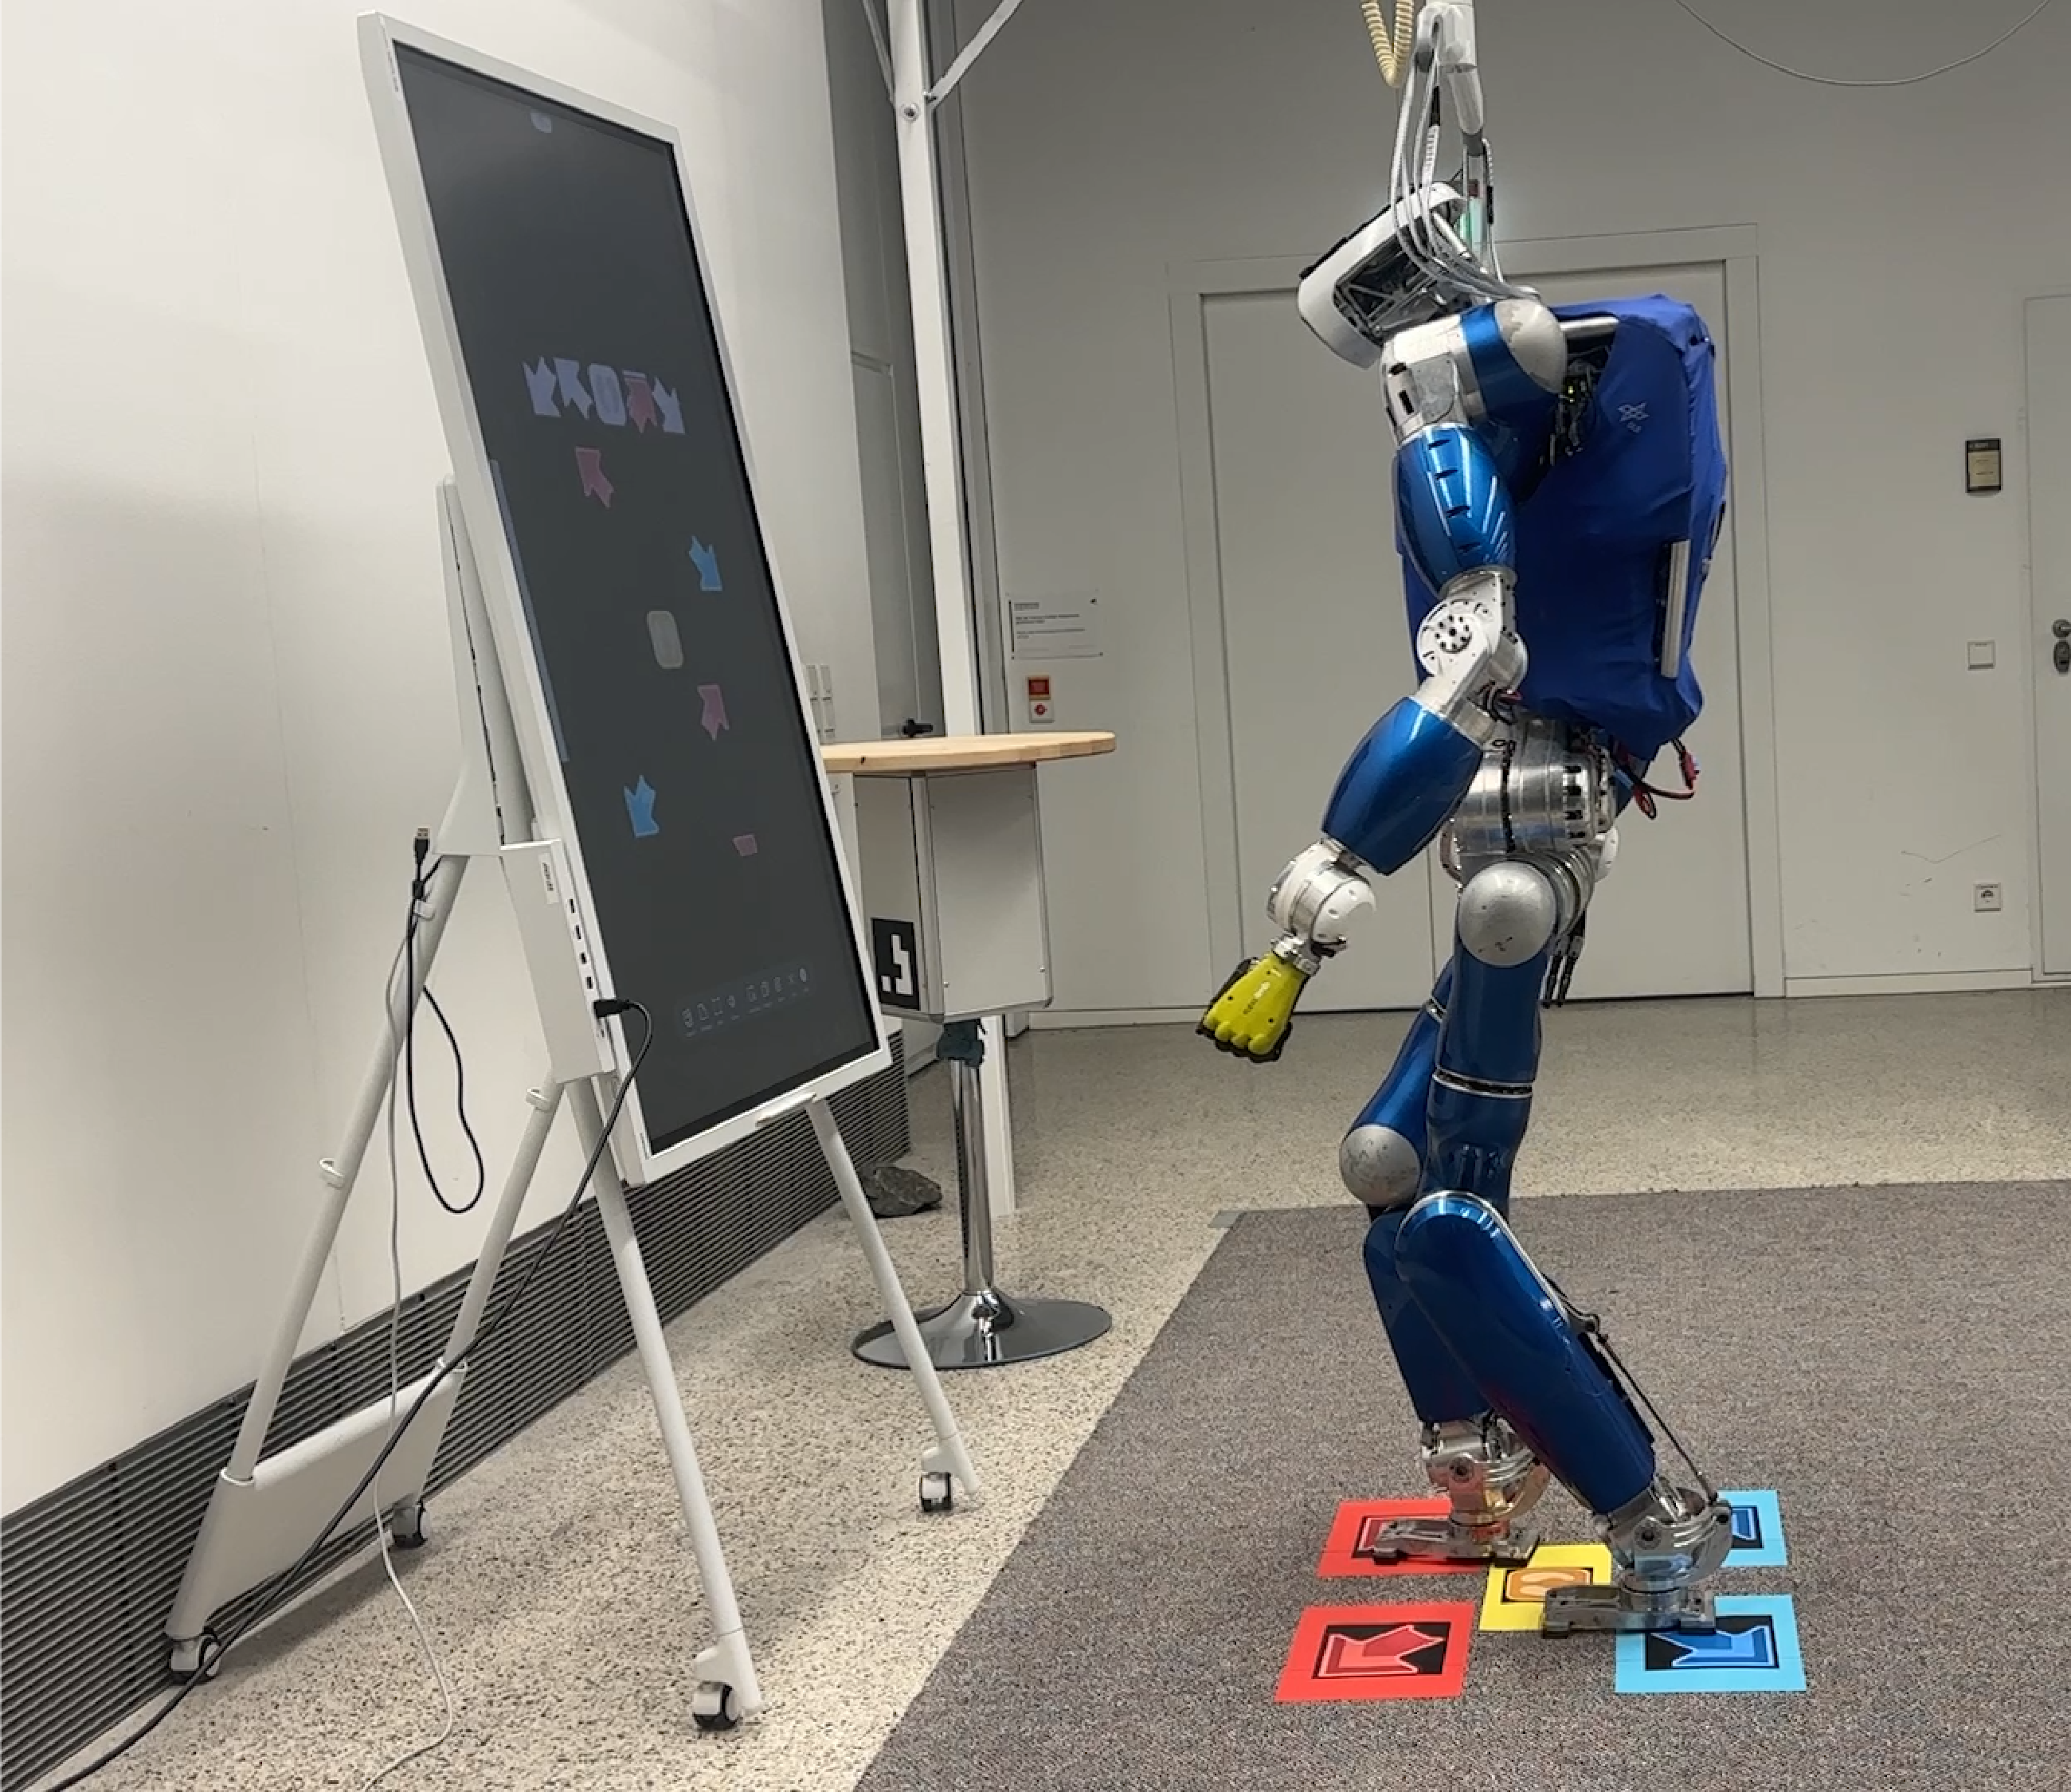
\includegraphics[width=0.75\linewidth]{Fig/main_fig.pdf}
    \caption{The humanoid robot performing the \textit{Pump It Up} scenario with real-time replanning based on step labels displayed on the screen.}
    \label{fig:main}
    \vspace{-4mm}
\end{figure}

Various methods address this coupled discrete-continuous planning problem.
A well-known graph-based methods such as A* \cite{chestnutt2003planning, chestnutt2005footstep, chestnutt2007adaptive}, ARA* \cite{hornung2012anytime}, and RRT \cite{xia2010global, liu2012hierarchical} formulate the problem as a graph search over discrete foot placement candidates. 
To capture the continuous nature of footstep planning within a searchable graph, these methods use a predefined action set that discretizes foot displacements in position and orientation.
These methods are widely used for their computational efficiency, enabling perception-based footstep planning~\cite{griffin2019footstep, michel2005vision}.
However, a small action set simplifies the search but limits feasible movements, whereas a larger action set better captures possible foot displacements but increases search complexity.
As a result, predefined actions can lead to suboptimal plans or failures when ideal footholds lie outside the discretized set.
Moreover, graph-based planners without predefined action sets have difficulty ensuring feasibility and often require long computation times in the enlarged continuous search space~\cite{marussi2025humanoid}.
In addition, their performance often depends on heuristic guidance, search priorities, and pruning strategies, making it sensitive to design choices.
\\
\indent
As an alternative to graph-based methods, optimization-based approaches handle both the discrete selection of contact surfaces and the continuous placement and orientation of each foot, typically formulated as mixed-integer program (MIP) \cite{dai2019global,driess2020deep,ponton2021efficient}.
However, their combinatorial complexity makes them computationally demanding and limits real-time applicability.
Several efforts have improved efficiency, including convex mixed-integer quadratically-constrained quadratic
program (MIQCQP) reformulations \cite{deits2014footstep}, linear programming relaxations \cite{tonneau2020sl1m}, and L1-norm-based pruning strategies \cite{song2021solving}.
Despite this progress, achieving both optimality and real-time performance in footstep planning remains challenging.
\\
\indent
This paper proposes a \textit{graph-based optimization} approach to humanoid footstep planning within the  Graphs of Convex Sets (GCS) framework.
We first formulate a nonconvex QCQP that incorporates terrain representation, kinematic reachability constraints, and cost terms for desirable stepping behavior.
Next, we construct a mode-aware graph, where each node corresponds to locomotion mode and represents a feasible convex region, while each edge denotes a transition between nodes.
We then integrate the nonconvex QCQP formulation with this graph structure, yielding a mixed-integer nonconvex program (MINCP) in which discrete transitions are represented by binary variables and foot placements are modeled as continuous variables.
To cope with the nonconvexity, we apply a semidefinite programming (SDP) relaxation to obtain a convex approximation of the relationships between footsteps.
Within the GCS framework, the discrete variables are relaxed into continuous variables, resulting in a computationally efficient relaxed-mixed integer convex program (R-MICP) while maintaining a tight relaxation.
The resulting problem is represented as a Shortest Path Problem in GCS (SPP in GCS), combining the computational efficiency of graph search with the solution quality of optimization-based approaches.
In this formulation, solving the convex relaxation does not require an initial discrete path or initial foot-placement values~\cite{marcucci2024shortest,marcucci2023motion}.
The main contributions of this work are summarized as follows:
\begin{itemize}
    \setlength\itemsep{0.5em}
    \item A novel unified footstep planning framework that simultaneously determines the discrete stepping sequence and the continuous placement of all footsteps.
    \item High-quality, initialization-independent footstep planning within real-time budgets. 
    \item Real-world validation on a humanoid robot, demonstrating applicability to rhythm-based stepping tasks under strict timing constraints.
\end{itemize}

\section{Preliminaries}

In this section, we briefly review the main background concepts underlying our approach.

\subsection{Shortest Path Problem in Graph of Convex Sets}
\label{sec:spp_gcs}

A GCS is defined as a directed graph $G = (\mathcal{V}, \mathcal{E})$ with a vertex set $\mathcal{V}$ and an edge set $\mathcal{E} \subseteq \mathcal{V}^2$. 
Each vertex $v \in \mathcal{V}$ is associated with a convex set $\mathcal{X}_v$, a variable $x_v \in \mathcal{X}_v$, and a convex cost function \( \ell_v(x_v) \ge 0 \). 
Additionally, each edge \( e = (u, v) \in \mathcal{E} \), with source vertex \(u\) and target vertex \(v\), is associated with a convex cost function \( \ell_e(x_u,x_v) \ge 0 \) and convex constraints of the form \( (x_u, x_v) \in \mathcal{X}_e \).
A path in the graph \( G \) is a sequence of distinct vertices that connects a source vertex \( s \in \mathcal{V} \) to a target vertex \( t \in \mathcal{V} \).  
Let \( \mathcal{P} \) denote the set of all such feasible \( s\text{–}t \) paths, and let \( \mathcal{E}_p \) denote the subset of edges traversed along path \( p \in \mathcal{P} \).  
The SPP in GCS is then expressed as detailed in~\cite{marcucci2024shortest}:
\begin{equation}
\begin{aligned}
\min_{p \in \mathcal{P}} \quad
& \sum_{v \in p} \ell_v(x_v) + \sum_{e\in\mathcal{E}_p} \ell_e(x_u,x_v) \\
\text{s.t.}\quad
& x_v \in \mathcal{X}_v,\! \forall v \in p,\!
  (x_u,x_v) \in \mathcal{X}_e,\! \forall e=(u,v)\in\mathcal{E}_p.
\end{aligned}
\label{eq:sppGCS}
\end{equation}
This formulation introduces binary variables that indicate whether each edge is selected along the path. 
Relaxing these binary variables to continuous ones yields the R-MICP, whose objective value provides a lower bound on that of the original MICP. 
Let \( C_{\text{relax}} \) and \( C_{\text{opt}} \) are objective values of the R-MICP and the original MICP, respectively. 
To recover a feasible solution to the original problem, a discrete path is selected from the relaxed edge values. 
Once the path is fixed, the continuous variables associated with the selected vertices and edges remain to be optimized, yielding a convex program with objective value denoted by \( C_{\text{round}} \).
These objective values satisfy \( C_{\text{relax}} \leq C_{\text{opt}} \leq C_{\text{round}} \).
Using these, the optimality gap \( \delta_{\text{opt}} \) and the relaxation gap \( \delta_{\text{relax}} \) are defined as
\begin{equation}\label{eq:relax_gap_def}
    \delta_{\text{opt}} = \frac{C_{\text{round}} - C_{\text{opt}}}{C_{\text{opt}}}
    \leq \delta_{\text{relax}} = \frac{C_{\text{round}} - C_{\text{relax}}}{C_{\text{relax}}}.
\end{equation}
\noindent
Thus, \( \delta_{\text{relax}} \) serves as an upper bound on \( \delta_{\text{opt}} \), providing an indirect measure of solution quality. A smaller \( \delta_{\text{relax}} \) indicates a tighter relaxation and suggests that the recovered solution is closer to the optimum of the original MICP~\cite{marcucci2023motion}.

\subsection{Semidefinite Programming Relaxation of Nonconvex Quadratically Constrained Quadratic Programs}
\label{sec:SDP}
To convexify nonconvex QCQPs, SDP relaxation and related tightening techniques are  employed \cite{yang2025new,sherali2013reformulation}.
Let \( y \in \mathbb{R}^n \), and define \( x := [\,1 \;\; y^\top\,]^\top \). Then, a nonconvex QCQP in homogeneous form can be expressed as
\begin{equation}
\begin{aligned}
    \min_{x}\quad     & x^\top Q_0 x \\
    \text{s.t.}\quad  & x^\top Q_i x \ge 0,\ \forall i=1,\dots,l,\quad A x \ge 0,
\end{aligned}
\label{eq:qcqp}
\end{equation}
\noindent where $A \in \mathbb{R}^{m \times (n+1)}$ and $Q_i \in \mathbb{R}^{(n+1) \times (n+1)}$ for $i = 0, \dots, l$.
The nonconvex QCQP in~\eqref{eq:qcqp} can be relaxed into the following semidefinite program:
\begin{equation}
\begin{aligned}
    \min_{X \succeq 0} \quad & \mathrm{tr}(Q_0 X) \\
    \text{s.t.} \quad & \mathrm{tr}(Q_i X) \geq 0,\; \forall i = 1, \dots, l \\
    & A X e_1 \geq 0,\; A X A^\top \geq 0,\;
    X = \begin{bmatrix} 1 & y^\top \\ y & Y \end{bmatrix} \succeq 0,
\end{aligned}
\label{eq:sdp}
\end{equation}
\noindent where \( e_1 \) is the \((n+1)\) dimensional vector with 1 in the first entry and 0 elsewhere.
If rank of \( X \) is one, i.e., \( X = x x^\top \), the problem~\eqref{eq:sdp} is equivalent to the original nonconvex QCQP~\eqref{eq:qcqp}.

\begin{figure*}[t]
  \centering
  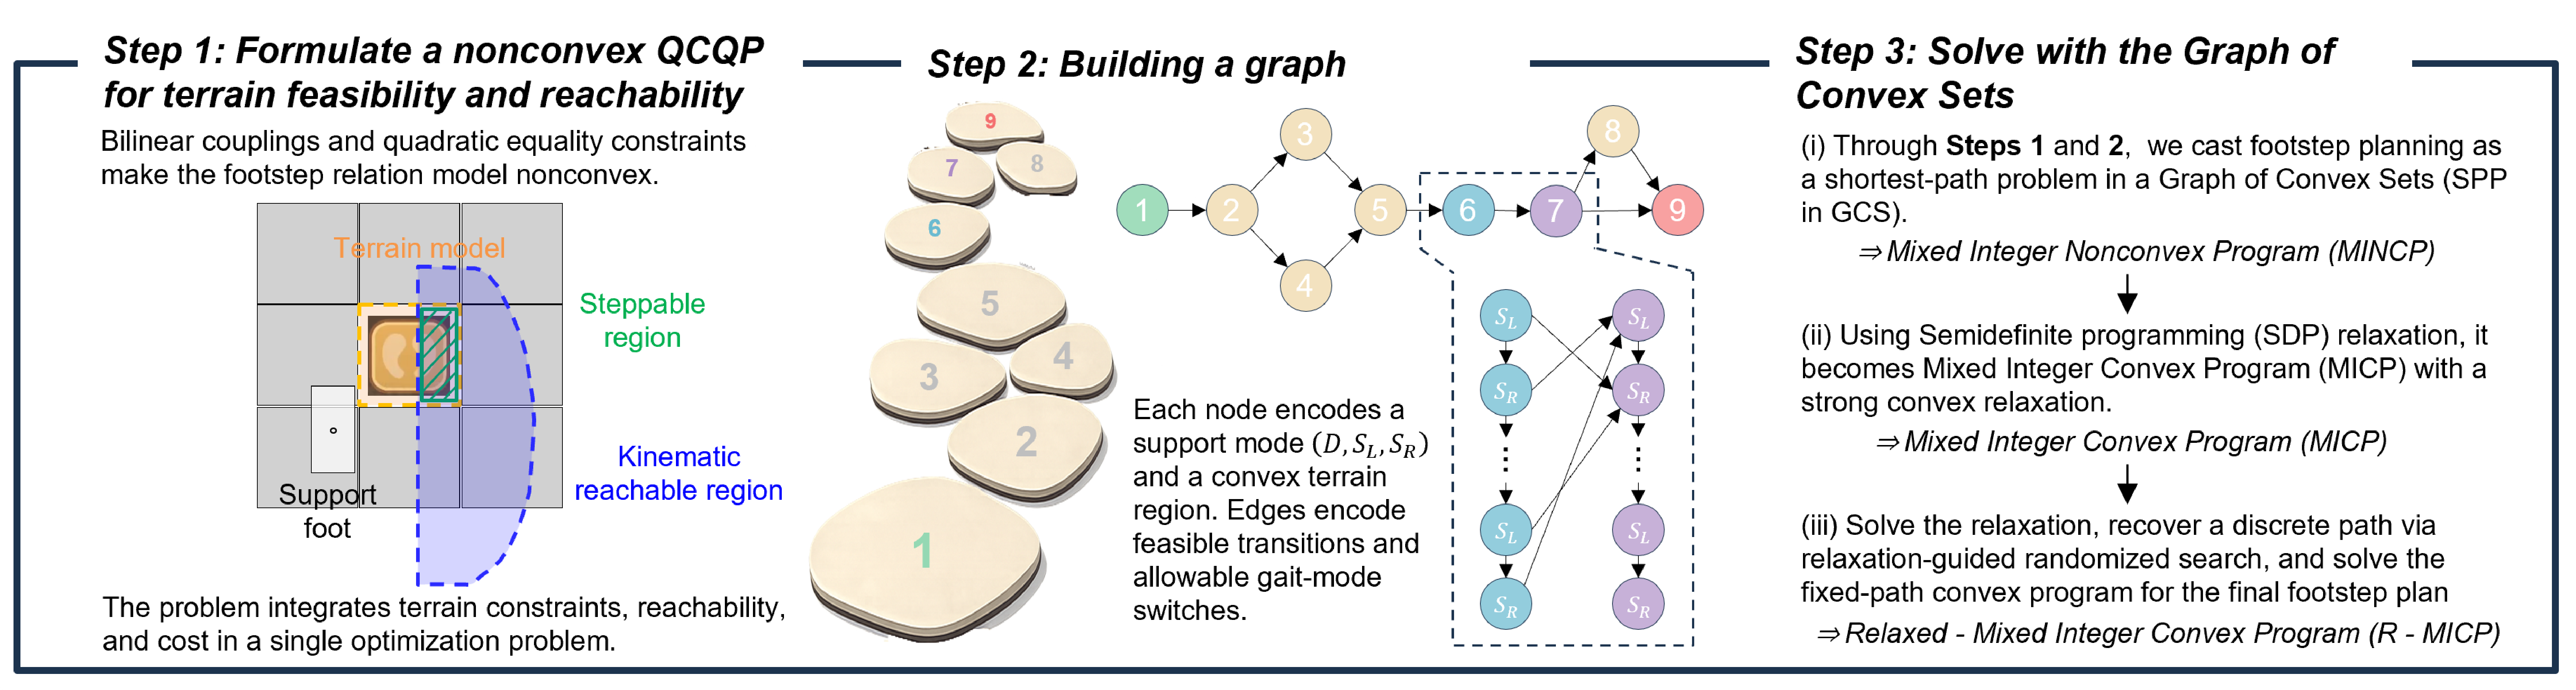
\includegraphics[width=1.00\textwidth]{Fig/Overview_method.pdf}
  \vspace{-6mm}
    \caption{
    Overview of the proposed planning pipeline.
    The method first models feasible footstep relations as a nonconvex QCQP, then builds a mode-aware graph over terrain regions and support phases.
    The resulting GCS problem is solved through convex relaxation, path recovery, and fixed-path refinement.
    }
  \label{fig:Overview_method}
  \vspace{-3mm}
\end{figure*}

\section{Method}

We formulate footstep planning as a nonconvex QCQP over continuous footstep configurations.
To handle the combinatorial structure of stepping decisions, we embed this formulation into a graph in which each node corresponds to a convex region associated with a locomotion mode and each edge encodes a feasible transition between nodes.
This allows us to cast the problem as a SPP in GCS framework.
Within this framework, we solve the resulting problem through relaxation and path recovery, followed by a convex optimization with the path fixed to compute the final footstep plan.
Fig.~\ref{fig:Overview_method} summarizes the overall pipeline.

\subsection{Formulating a nonconvex Quadratically Constrained Quadratic Program}

We aim to compute a sequence of footstep configurations connecting a start configuration to a goal configuration while satisfying terrain-feasibility and kinematic reachability constraints and minimizing task-specific costs.
At step $k$, the pose of each foot $F \in \{L,R\}$, with \(L\) and \(R\) denoting the left and right foot, is represented by a 5D vector $\mathbf{q}_k^F = (x_k^F, y_k^F, z_k^F, \cos\theta_k^F, \sin\theta_k^F)$, and the full footstep configuration is written as $\mathbf{s}_k = (\mathbf{q}_k^L, \mathbf{q}_k^R)$.
Note that, rather than parameterizing orientation by $\theta$, we use its sine and cosine components as decision variables, avoiding nonconvex trigonometric functions in the formulation.
The initial and goal configurations are fixed and denoted by $\mathbf{s}_{\text{init}}$ and $\mathbf{s}_{\text{goal}}$, while the intermediate configurations are decision variables with the same parameterization.
Each footstep is constrained to lie in one of a set of convex regions representing collision-free and supportable terrain areas.
These regions are derived from the environment geometry and restrict footsteps to physically feasible locations.
Throughout the sequence, the phase transitions among left- and right-single-support and double-support phases, inducing phase-dependent constraints between consecutive configurations.
Accordingly, we impose constraint sets for each support transition to ensure kinematic feasibility.

\subsubsection{Terrain Representation}
To model terrain feasibility, we represent the environment as convex regions that describe obstacle-free and supportable areas for foot placement.
While various methods exist for decomposing feasible spaces into convex sets~\cite{Deits2015Computing, werner2024faster}, we manually construct these regions in our experiments, as the considered test terrains have structured and known support regions.
We define the planar position of foot $F$ at step $k$ as $p_k^F = [x_k^F\;\; y_k^F]^\top$.
Formally, each region $g \in \{1,\dots,G\}$ is described by the linear inequality constraints
\begin{equation}
    A_g p_k^F \le b_g
    \label{eq:terrain_region}
\end{equation}
for all relevant footsteps.
The matrix $A_g$ and vector $b_g$ define the boundary of region $g$ in the planar space.
Because each convex region lies on a support surface, the height $z_k^F$ is determined by the terrain once the planar position $p_k^F$ is fixed.

\subsubsection{Reachability Constraints}
To ensure kinematic feasibility between footsteps, we impose constraints on step length, heading change, and relative foot placement consistency.
We constrain the next swing-foot placement to remain within a maximum step length from the current support foot:
\begin{equation}
    \|p_{k+1}^{\mathrm{sw}} - p_k^{\mathrm{sup}}\|_2 \le d_{\max},
\label{eq:convex}
\end{equation}
\noindent where $p_k^{\mathrm{sup}}$ and $p_{k+1}^{\mathrm{sw}}$ denote the support-foot position at step $k$ and the next swing-foot landing position, respectively, and $d_{\max}$ is the maximum allowable step length.
\\
\indent
To account for terrain-height transitions, we impose
\begin{equation}
-h_{\mathrm{down}}
\le z_{k+1}^{\mathrm{sw}}-z_k^{\mathrm{sup}}
\le h_{\mathrm{up}},
\label{eq:vertical_reachability}
\end{equation}
where $h_{\mathrm{up}}$ and $h_{\mathrm{down}}$ denote the maximum allowable step-up and step-down heights, respectively.
\\
\indent
For orientation, we introduce a unit direction vector $r_k^F = [\cos\theta_k^F\;\; \sin\theta_k^F]^\top$ to represent the yaw angle of each footstep.
To ensure that $r_k^F$ represents a valid yaw angle, we constrain it to lie on the unit circle.
We also limit heading changes between successive placements of the same foot to prevent large rotations.
These constraints are imposed for both feet:
\begin{equation}
    \|r_k^F\|_2^2 = 1,\quad (r_k^F)^\top r_{k+1}^F \ge \cos(\Delta\theta_{\max}),
\label{eq:nonconvex_1}
\end{equation}
\noindent where $\Delta\theta_{\max}$ denotes the maximum allowable yaw change between consecutive placements of the same foot.
\\
\indent
To maintain a consistent stepping geometry relative to the heading direction, we impose additional constraints between alternating footsteps.
The next right foot is constrained to lie on the right side of the heading direction of the current left foot, while the next left foot is constrained to lie on the left side of the heading direction of the current right foot as follows:
\begin{equation}
    \cos\theta_k^{L}\,(y_{k+1}^{R} - y_k^{L}) - \sin\theta_k^{L}\,(x_{k+1}^{R} - x_k^{L}) \le 0
\label{eq:nonconvex_3}
\end{equation}
\begin{equation}
    \cos\theta_k^{R}\,(y_{k+1}^{L} - y_k^{R}) - \sin\theta_k^{R}\,(x_{k+1}^{L} - x_k^{R}) \ge 0.
\label{eq:nonconvex_4}
\end{equation}
\indent
In addition, we encourage directional consistency by constraining the next placement of the same foot to lie on the line defined by its previous position and heading.
Let $(r_k^F)^\perp = [-\sin\theta_k^F\;\; \cos\theta_k^F]^\top$ denote a vector perpendicular to $r_k^F$.
The following constraint is imposed for both feet:
\begin{equation}
    ((r_k^F)^\perp)^\top (p_{k+1}^F - p_k^F) = 0.
\label{eq:nonconvex_5}
\end{equation}
This constraint suppresses inward steps that may cause knee collision and overly wide steps that may lead to instability.
It may be omitted or reformulated for other platforms.

\subsubsection{Cost Function}
The cost function promotes efficient footstep plans while regularizing the resulting sequence toward stable and natural foot placements.
It consists of four convex components, described below.
The total cost is defined as
\begin{equation}
J=\sum_{k=0}^{N-1}\!\bigl[
L(\mathbf{s}_k,\mathbf{s}_{k+1})+R(\mathbf{s}_k,\mathbf{s}_{k+1})
+D(\mathbf{s}_k,\mathbf{s}_{k+1})+T(\mathbf{s}_k)
\bigr],
\label{eq:total_cost}
\end{equation}
\noindent where the first term \(L\) encourages efficient footstep transitions by penalizing both the planar displacement and the vertical height variation between successive placements of each foot:
\begin{equation}
L(\mathbf{s}_k,\mathbf{s}_{k+1})
= k_l\sum_{F\in\{L,R\}}
\bigl(\|p_{k+1}^F-p_k^F\|_2+|z_{k+1}^F-z_k^F|\bigr),
\end{equation}
\noindent
while the second term \(R\) promotes consistency between the foot orientation and the stepping direction.
It penalizes the mismatch between each foot's orientation vector and the scaled displacement of the midpoint between the two feet:
\begin{equation}
    R(\mathbf{s}_k, \mathbf{s}_{k+1})
    = k_r \sum_{F \in \{L,R\}} \left\| r_k^F - \bigl(c_{k+1} - c_k\bigr)/s_r \right\|_2,
\label{eq:rotation_cost}
\end{equation}
\noindent where \(c_k = \frac{p_k^L + p_k^R}{2}\) is the center between the feet at step \(k\), and \(s_r\) normalizes the average stepping direction.
The third term \(D\) penalizes deviations from a preferred lateral offset \(s_d\) to avoid unnaturally narrow steps:
\begin{equation}
\begin{aligned}
D(\mathbf{s}_k, \mathbf{s}_{k+1}) =\;
&\, k_d \left\| \left(c_k - p_{k+1}^L\right) - s_d (r_k^L)^\perp \right\|_2 \\
&+ k_d \left\| \left(p_{k+1}^R - c_k\right) - s_d (r_k^R)^\perp \right\|_2 .
\end{aligned}
\label{eq:model_cost}
\end{equation}
Here, \(s_d\) denotes the desired lateral offset between the feet, chosen based on the robot's physical design.
Lastly, the fourth term \(T(\mathbf{s}_k)=k_t n_{\mathrm{step}}\) penalizes the number of selected footstep transitions, where \(n_{\mathrm{step}}\) denotes the number of transitions selected by the path.
Here, \(N\) defines the maximum planning horizon, while \(n_{\mathrm{step}}\) represents the actual number of footsteps used in the plan.
This encourages shorter step sequences.
The weights \(k_l, k_r, k_d,\) and \(k_t\) penalize path length, rotation alignment, lateral foot separation, and step count, respectively.

\subsubsection{Optimization Problem}
Combining the terrain representation, reachability constraints, and the cost function defined in~\eqref{eq:total_cost}, we formulate the problem as a nonconvex QCQP.
Given fixed start and goal configurations for both feet and a planning horizon \(N\), we seek a sequence of step configurations $\{\mathbf{s}_k\}_{k=0}^{N}$ that minimizes the total cost $J$:
\begin{equation}
\label{eq:footstep_qcqp}
\begin{aligned}
\min_{\{\mathbf{s}_k\}_{k=0}^{N}} \quad
& J \\
\text{s.t.}\
& \mathbf{s}_0 = \mathbf{s}_{\text{init}},\!
  \mathbf{s}_N = \mathbf{s}_{\text{goal}},\!
  \eqref{eq:convex}\text{--}\eqref{eq:nonconvex_5},\!
  \forall k = 0,\dots,N, \\
& p_k^L,\, p_k^R \in \bigcup_{g=1}^{G} \mathcal{X}_g,\!
  \forall k = 0,\dots,N-1,
\end{aligned}
\end{equation}
\noindent where each region is defined as \(\mathcal{X}_g = \{ p \in \mathbb{R}^2 \mid A_g p \le b_g \}\).
\indent This formulation is nonconvex due to quadratic equalities and bilinear terms, and it includes a discrete component through the disjunctive region constraints.
This structure motivates the graph-based embedding in the following subsection.

\subsection{Building a Graph}
\label{sec:Buildingagraph}
\begin{figure}[t]
    \centering
    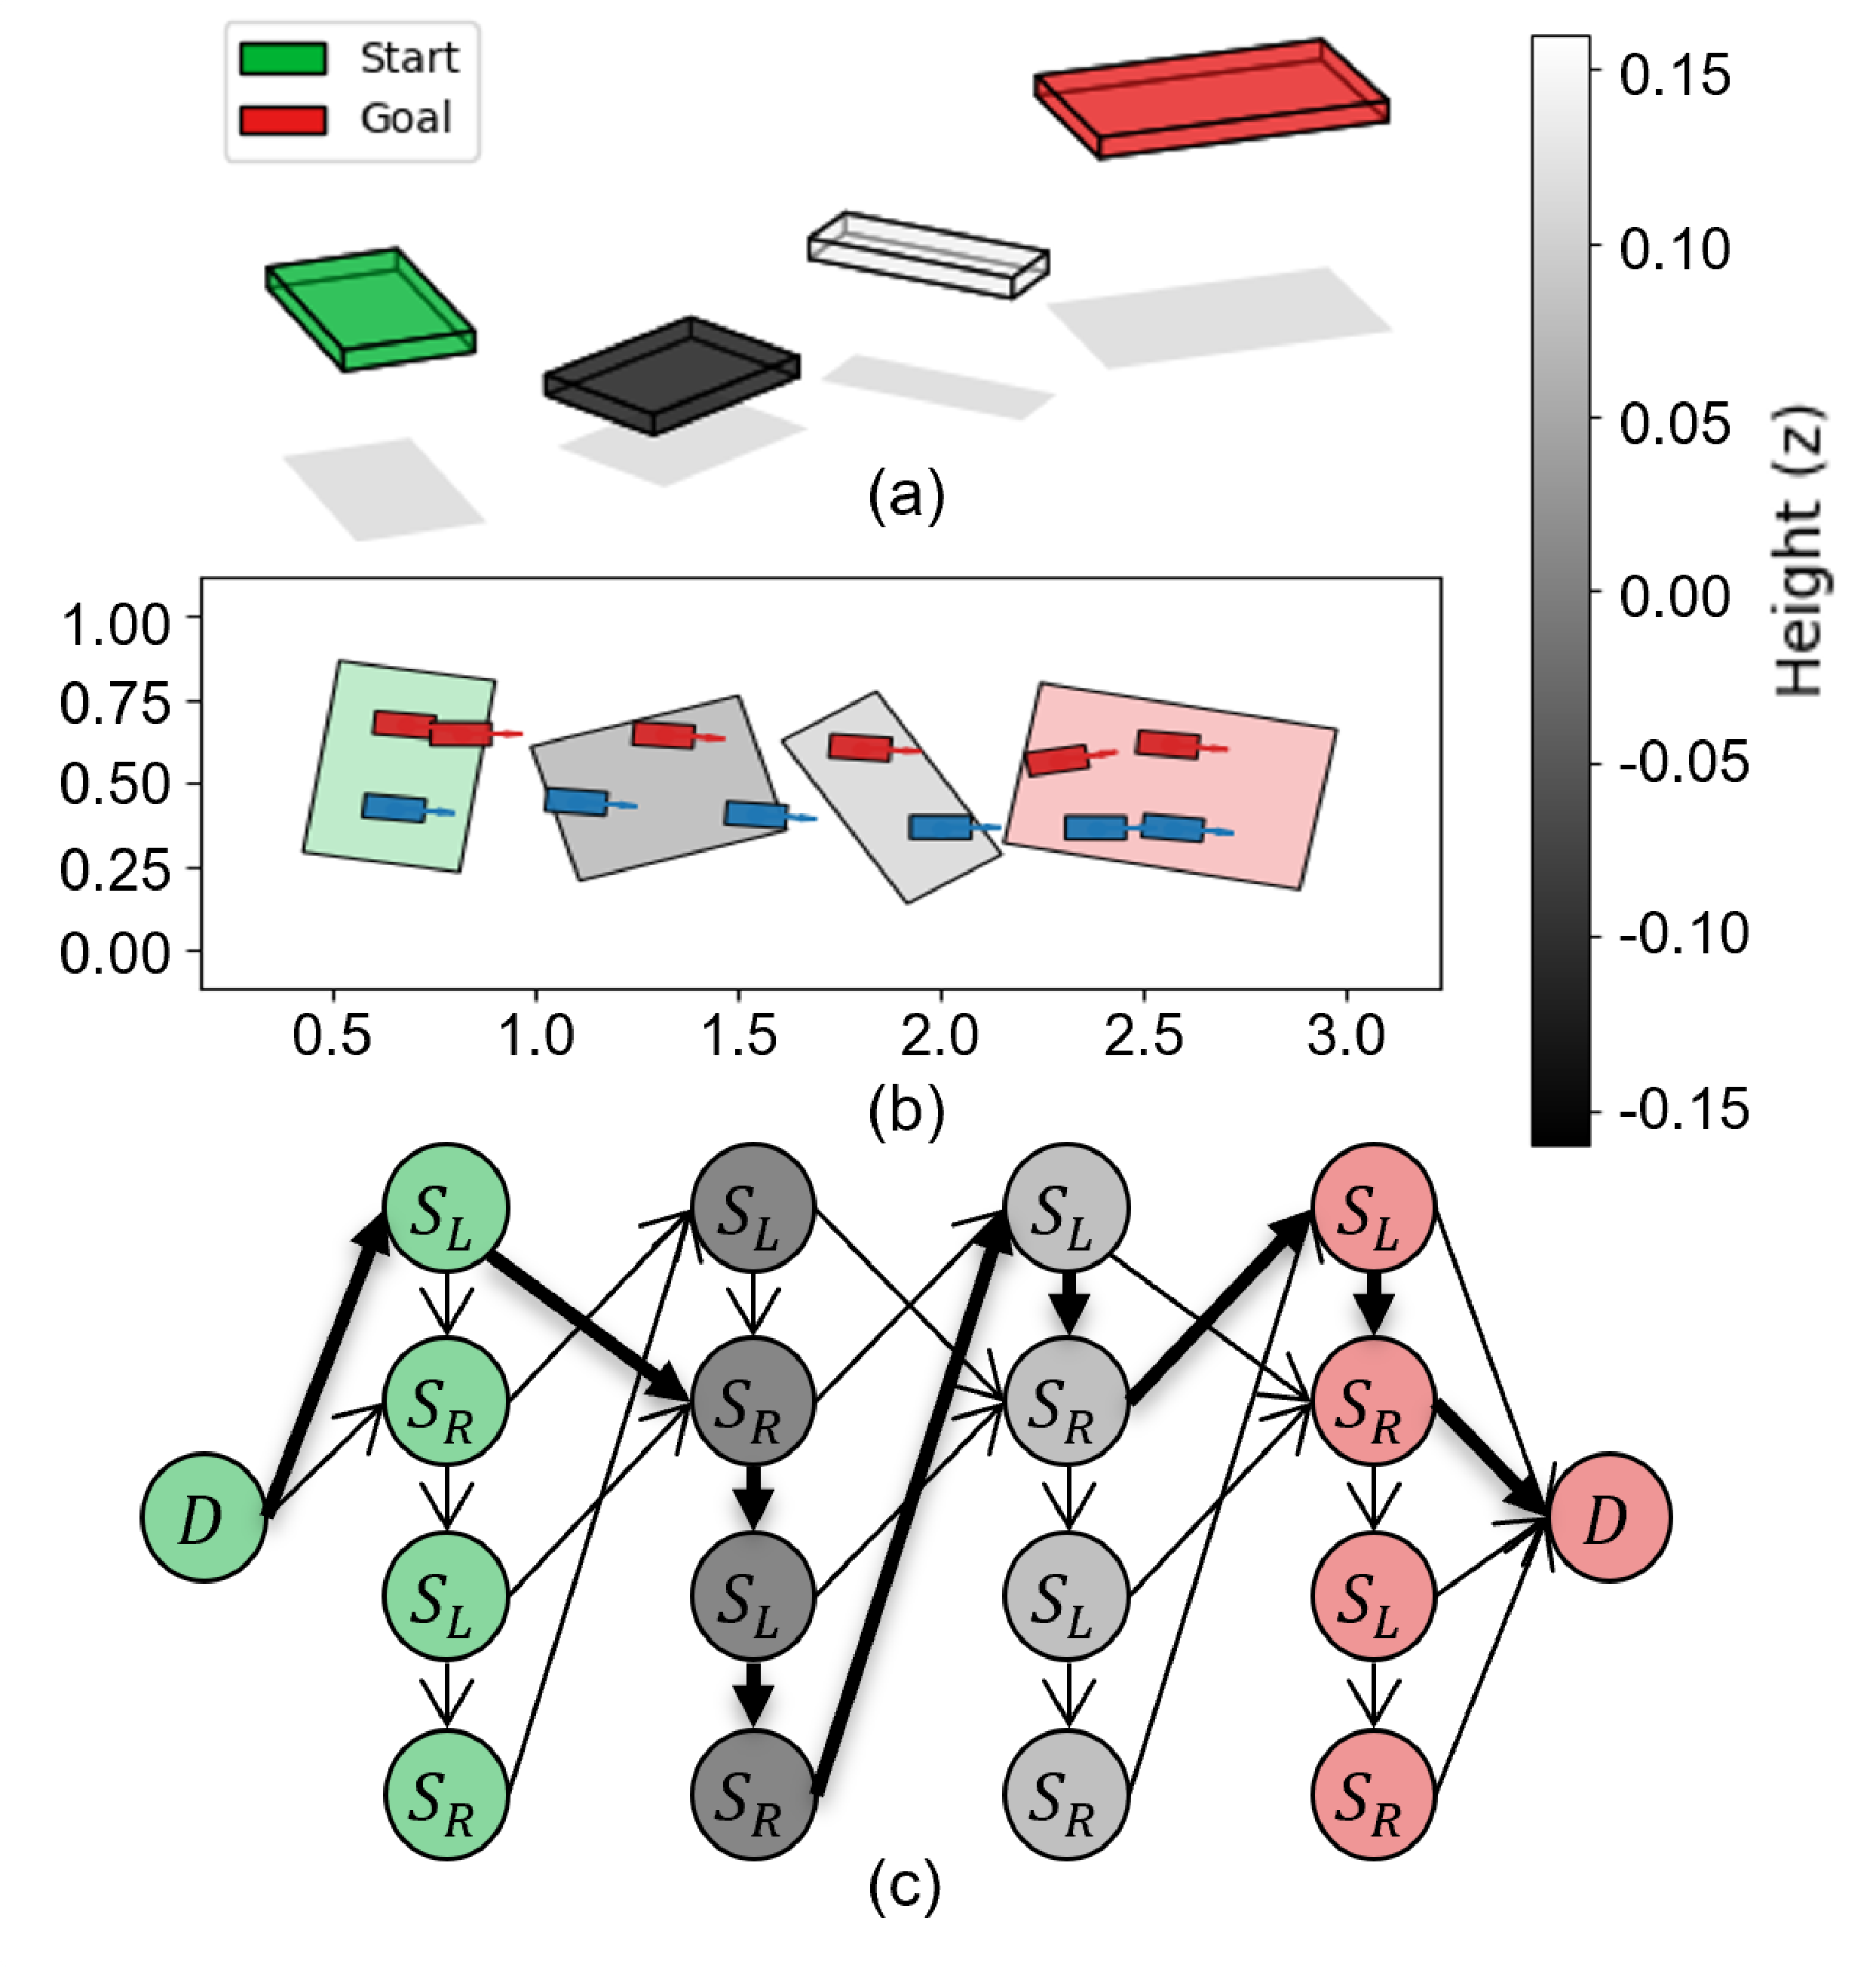
\includegraphics[width=0.75\linewidth]{Fig/Graph_explain.pdf}
    \vspace{-3mm}
    \caption{
    Example of a GCS formulation.
    (a) Randomly generated stepping-stone terrain with given start/goal configurations (height indicated by the color scale).
    (b) Top-down view of a footstep plan produced by our planner (red: left foot, blue: right foot).
    (c) Each node represents a region with mode $m_v\in\{D, S_L, S_R\}$, and the bold path indicates the selected edge sequence corresponding to (b).
    }
    \label{fig:Graph_explain}
    \vspace{-2mm}
\end{figure}
Each vertex in the graph is defined by a geometric region and a support mode as shown in Fig.~\ref{fig:Overview_method}.
The region corresponds to a convex foot placement area on the terrain, and the mode indicates whether the robot is in double support ($D$), left-foot single support ($S_L$), or right-foot single support ($S_R$).
We specify the start and goal footstep poses and partition the terrain into convex regions.
To allow the robot to step on the same region multiple times, each region is duplicated a number of times.
The number of duplicates is chosen according to the size of the region, so that larger foothold regions are assigned more copies and can accommodate a richer set of candidate transitions.
Each vertex $v \in \mathcal{V}$ is therefore defined by a convex region 
$X_v \subset \mathbb{R}^2$ and a support mode 
$m_v \in \{D, S_L, S_R\}$.
\\
\indent
As illustrated in Fig.~\ref{fig:Graph_explain}, one possible assignment follows a structured alternating pattern over $S_L$ and $S_R$, with $D$ included only at start and goal poses to represent double-support transitions.
The edges $e \in \mathcal{E}$ capture feasible transitions between vertices.
Rather than fully connecting all duplicated vertices, we introduce edges only for mode-compatible transitions that preserve the intended support-phase progression and provide additional geometric reachability, thereby avoiding an overly dense graph.
A path in the graph encodes a physically valid sequence of steps, support transitions, and foot placements.

\subsection{Solving with the Graph of Convex Sets}
\label{sec:solve_gcs}
\begin{table}[t]
\vspace{-3mm}
\centering
\caption{Problem reformulations in the proposed workflow.}
\label{tab:problem_transformation}
\footnotesize
\setlength{\tabcolsep}{4pt}
\renewcommand{\arraystretch}{1.1}
\begin{tabularx}{\columnwidth}{l X l}
\toprule
\textbf{Current form} & \textbf{Key operation} & \textbf{Resulting form} \\
\midrule
Nonconvex QCQP & GCS graph embedding & MINCP \\
MINCP & Tightened SDP relaxation & MICP \\
MICP & Binary relaxation & R-MICP \\
\bottomrule
\end{tabularx}
\vspace{-5mm}
\end{table}
Combining the nonconvex QCQP~\eqref{eq:footstep_qcqp} with the mode-aware graph, we cast the footstep planning problem as a SPP in GCS.
For each directed edge $e=(u,v)\in\mathcal E$ and foot $F\in\{L,R\}$, we introduce the following edge-level decision variables:
\begin{equation}
y_e,\quad \xi_e,\quad X_{e,F}^{(5)}\in\mathbb S_+^5,\quad X_{e,F}^{(7)}\in\mathbb S_+^7.
\label{eq:gcs_decision_variables}
\end{equation}
Here, $y_e$ is the binary edge-selection variable, and $\xi_e$ collects edge-local variables, including the edge-end copies $\mathbf{q}_{e,F}^{-}$ and $\mathbf{q}_{e,F}^{+}$ of the 5D footstep state and additional auxiliary variables used in the convex reformulation.
For edge-local variables, the superscripts \( - \) and \( + \) denote the source and target ends of edge \(e\), respectively, whereas \(\mathbb S_+^n\) denotes positive semidefinite matrices.
To convexify the nonconvex terms via SDP relaxation, we use the lifted matrices $X_{e,F}^{(5)}$ and $X_{e,F}^{(7)}$.
These variables are linked across adjacent edges through continuity constraints so that the selected $s$--$t$ path defines a globally consistent footstep sequence.
Table~\ref{tab:problem_transformation} summarizes the sequence of reformulations used in the proposed workflow.
We first obtain a graph-embedded MINCP, then convexify its edge-local nonconvex constraints through a lifted SDP relaxation, and finally solve a relaxed formulation followed by path recovery.

\subsubsection{From nonconvex QCQP to a graph-embedded MINCP}

Using the variables~\eqref{eq:gcs_decision_variables}, we collect the graph-consistency constraints into the set $\mathcal F_{\mathrm{GCS}}$.
These include the standard GCS flow constraints, the continuity constraints on the edge-local footstep states, and the boundary conditions at the source and target.
Let $\delta^+(v)$ and $\delta^-(v)$ denote the sets of outgoing and incoming edges of vertex $v$.
The flow constraints are
\begin{subequations}\label{eq:gcs_flow}
\begin{align}
\sum_{e\in\delta^+(s)} y_e &= 1, \qquad
\sum_{e\in\delta^-(t)} y_e = 1, \label{eq:gcs_flow_st}\\
\sum_{e\in\delta^-(v)} y_e - \sum_{e\in\delta^+(v)} y_e &= 0,
\qquad \forall v\in\mathcal V\setminus\{s,t\}, \label{eq:gcs_flow_cons}\\
\sum_{e\in\delta^+(v)} y_e &\le 1,
\qquad \forall v\in\mathcal V\setminus\{s,t\}. \label{eq:gcs_outflow_cap}
\end{align}
\end{subequations}
\indent
The edge-local footstep states are linked across adjacent edges through continuity and boundary conditions:
\begin{equation}\label{eq:gcs_state_linking}
\begin{alignedat}{3}
\sum_{e\in\delta^-(v)} \mathbf{q}_{e,F}^{+}
&= \sum_{e\in\delta^+(v)} \mathbf{q}_{e,F}^{-},
\, \forall v\in\mathcal V\setminus\{s,t\},
\; F\in\{L,R\},\\
\mathbf{q}_{e,L}^{-} &= y_e\, \mathbf{q}_{\text{init}}^{L},
\;
\mathbf{q}_{e,R}^{-} = y_e\, \mathbf{q}_{\text{init}}^{R},
\; \forall e\in\delta^+(s),\\
\mathbf{q}_{e,L}^{+} &= y_e\, \mathbf{q}_{\text{goal}}^{L},
\;
\mathbf{q}_{e,R}^{+} = y_e\, \mathbf{q}_{\text{goal}}^{R},
\; \forall e\in\delta^-(t).
\end{alignedat}
\end{equation}
\noindent
These constraints connect the footstep states across adjacent edges and match the source and target states to the initial and goal configurations.
We collect the convex edge-local constraints into the set $\mathcal C_e$.
This set includes the terrain-feasibility constraints induced by~\eqref{eq:terrain_region} and the convex reachability bounds in~\eqref{eq:convex} and~\eqref{eq:vertical_reachability}.
It includes mode-dependent stance-consistency and support-surface constraints from the graph embedding.
These constraints are written in perspective form with respect to $y_e$, so that inactive edges carry no active contribution.
For example, the terrain-feasibility constraint in~\eqref{eq:terrain_region} becomes \(A_r p_{e,F}^{+} \le y_e b_r\), where $p_{e,F}^{+}$ is the planar position of foot $F$ at the target end of edge $e$.
When $y_e=1$, this reduces to~\eqref{eq:terrain_region}; when $y_e=0$, it becomes inactive in conjunction with the zero-state constraints imposed on inactive edges.
Together, $\mathcal F_{\mathrm{GCS}}$ and $\mathcal C_e$ define the graph-embedded MINCP.

\subsubsection{Lifted SDP relaxation of the edge-local nonconvex constraints}

The graph-embedded MINCP contains edge-local nonconvex constraints arising from~\eqref{eq:nonconvex_1}--\eqref{eq:nonconvex_5}.
To relax these terms, we used lifted semidefinite variables and collect the resulting lifted edge-local constraints associated with edge $e$ into the set $\mathcal S_e$.
For each foot $F\in\{L,R\}$, we define
\begin{equation}\label{eq:lifted_blocks}
\begin{aligned}
\eta_{e,F}^{(5)} &= [\,1,\ c_{e,F}^{-},\ s_{e,F}^{-},\ c_{e,F}^{+},\ s_{e,F}^{+}\,]^{\top},\\
\eta_{e,F}^{(7)} &= [\,1,\ x_{e,F}^{-},\ y_{e,F}^{-},\ c_{e,F}^{-},\ s_{e,F}^{-},\ x_{e,F}^{+},\ y_{e,F}^{+}\,]^{\top},
\end{aligned}
\end{equation}
\noindent where \(x_{e,F}^{\pm}\) and \(y_{e,F}^{\pm}\) are the planar position components, while \(c_{e,F}^{\pm}\) and \(s_{e,F}^{\pm}\) are the cosine and sine yaw components of edge \(e\).
The lifted blocks $X_{e,F}^{(5)}$ and $X_{e,F}^{(7)}$ correspond to SDP relaxations of $\eta_{e,F}^{(5)}{\eta_{e,F}^{(5)}}^{\top}$ and $\eta_{e,F}^{(7)}{\eta_{e,F}^{(7)}}^{\top}$, respectively.
They are used to impose orientation-only quadratic constraints and position--orientation bilinear terms in the lifted space.
In practice, the entries of $\eta_{e,F}^{(5)}$ and $\eta_{e,F}^{(7)}$ are chosen according to the structure of the corresponding edge-local nonconvex constraint.
Following the SDP relaxation in~\eqref{eq:sdp}, the original nonconvex relations are replaced by positive-semidefinite constraints together with linear constraints on the lifted entries.
\\
\indent
To tighten the relaxation, we impose coupling constraints between entries of the lifted blocks and add Reformulation-Linearization Technique (RLT) constraints based on variable bounds.
Here, \([X]_{ij}\) denotes the \((i,j)\)-th entry of matrix \(X\).
For example, since $c_{e,F}^{-}$ appears in both $\eta_{e,F}^{(5)}$ and $\eta_{e,F}^{(7)}$ in~\eqref{eq:lifted_blocks}, the corresponding lifted entries are coupled as
\begin{equation}
\left[X_{e,F}^{(5)}\right]_{12} = \left[ X_{e,F}^{(7)}\right]_{14}.
\label{eq:coupling_example}
\end{equation}
Similar constraints are imposed on the other shared orientation-related entries.
For bounded bilinear products, we impose RLT constraints on the corresponding lifted entries.
For example, let $u=c_{e,F}^{-}$, $v=x_{e,F}^{+}$, and $w=\left[ X_{e,F}^{(7)}\right]_{46}$.
For $u\in[\underline u,\bar u]$ and $v\in[\underline v,\bar v]$, the RLT inequalities are
\begin{equation}\label{eq:rlt_example}
\begin{aligned}
w &\ge \underline u\, v + \underline v\, u - \underline u \underline v, \qquad
w \ge \bar u\, v + \bar v\, u - \bar u \bar v,\\
w &\le \bar u\, v + \underline v\, u - \bar u \underline v, \qquad
w \le \underline u\, v + \bar v\, u - \underline u \bar v.
\end{aligned}
\end{equation}
These inequalities bound the lifted product entry using only linear constraints and bounds on the underlying scalar variables.
We further strengthen the formulation using box bounds on scalar variables, diagonal caps on selected lifted entries, trace-based regularization of the lifted matrices, and mode-dependent geometric constraints.
After replacing the edge-local nonconvex constraints with these lifted convex constraints, the MINCP becomes a tightened MICP.

\subsubsection{Relaxed formulation and path recovery}

Applying binary relaxation to the tightened MICP yields the final R-MICP:
\begin{equation}
\label{eq:rmicp_compact_revised}
\begin{aligned}
\min_{\substack{y,\xi,\{X_{e,F}^{(5)}\},\{X_{e,F}^{(7)}\}}} \!
& \sum_{e\in\mathcal E} \tilde{\ell}_e(y_e,\xi_e) \\
\text{s.t.}\,
& (y,\xi)\in \mathcal F_{\mathrm{GCS}}, \! (y_e,\xi_e)\in \mathcal C_e, \! \forall e\in\mathcal E, \\
& (y_e,\xi_e,\{X_{e,F}^{(5)}\},\{X_{e,F}^{(7)}\})\in \mathcal S_e,
\! \forall e\in\mathcal E, \\
& y_e \in [0,1], \, \forall e\in\mathcal E .
\end{aligned}
\end{equation}
Here, $\tilde{\ell}_e(y_e,\xi_e)$ denotes the perspective form of the edge-local cost induced by~\eqref{eq:total_cost}, including the step-length, vertical-displacement, and step-penalty terms.
The notations \(\{X_{e,F}^{(5)}\}\) and \(\{X_{e,F}^{(7)}\}\) denote the collections of lifted matrices over all \(e\in\mathcal E\) and \(F\in\{L,R\}\).
The sets $\mathcal F_{\mathrm{GCS}}$, $\mathcal C_e$, and $\mathcal S_e$ collect the graph-consistency constraints, convex edge-local constraints, and lifted convex constraints, respectively.
\\
\indent
Solving the R-MICP yields relaxed edge values $\{y_e^\star\}_{e\in\mathcal E}$, which are used to recover a $s$--$t$ path.
We consider two recovery strategies: (i) a greedy strategy that prioritizes larger edge values and (ii) a probabilistic relaxation-guided search based on normalized relaxed edge weights.
The probabilistic strategy is implemented as a depth-first search with backtracking, where a parameter controls the exploration--exploitation.
For each candidate path $\mathcal P$, we fix the edge-selection variables and set all other edges to zero, yielding a convex subproblem.
Among all feasible recovered paths, we retain the one with the smallest objective value as the final footstep plan.

\section{Verification}

This section evaluates the reliability of the proposed planner on challenging stepping-stone terrains and its sensitivity to graph construction.
For a controllable-difficulty benchmark, we use a conditional variational autoencoder (CVAE)-based stepping-stone generator~\cite{kim2025high}.
We compare a graph-based method~\cite{griffin2019footstep}, an optimization-based method~\cite{deits2014footstep}, and the proposed method.
For a fair comparison, all planners use the same stone representation, feasibility constraints, and reachability limits.
A trial succeeds if the planner returns a feasible footstep sequence that reaches the goal within a tolerance.
We examine how vertex duplication and edge density affect success rate, computation time, and relaxation tightness.

\subsection{CVAE-based Terrain Generation}

We represent the relative transition between consecutive stones by a 6D delta vector encoding changes in center position, size, and yaw.
We construct 40,000 conditional samples \((c_t,X_t)\), where \(c_t=[X_{t-2},X_{t-1}] \in \mathbb{R}^{12}\) contains the previous two transitions and \(X_t \in \mathbb{R}^{6}\) is the current transition.
Using this dataset, we train a CVAE with latent dimension 8 to autoregressively generate \(X_t\) conditioned on \(c_t\).
Starting from two seed transitions, the generated sequence defines the stepping stones, with the first and last used as the start and goal.
Terrain difficulty is controlled by sampling \(z\sim\mathcal{N}(0,(1+\alpha)I)\), with \(\alpha\in\{0,0.5,1\}\).
Larger \(\alpha\) values yield more dispersed transitions in spacing, height, size, and yaw, producing increasingly irregular terrains.

\subsection{Evaluation of planners}

\begin{figure}[t]
    \centering
    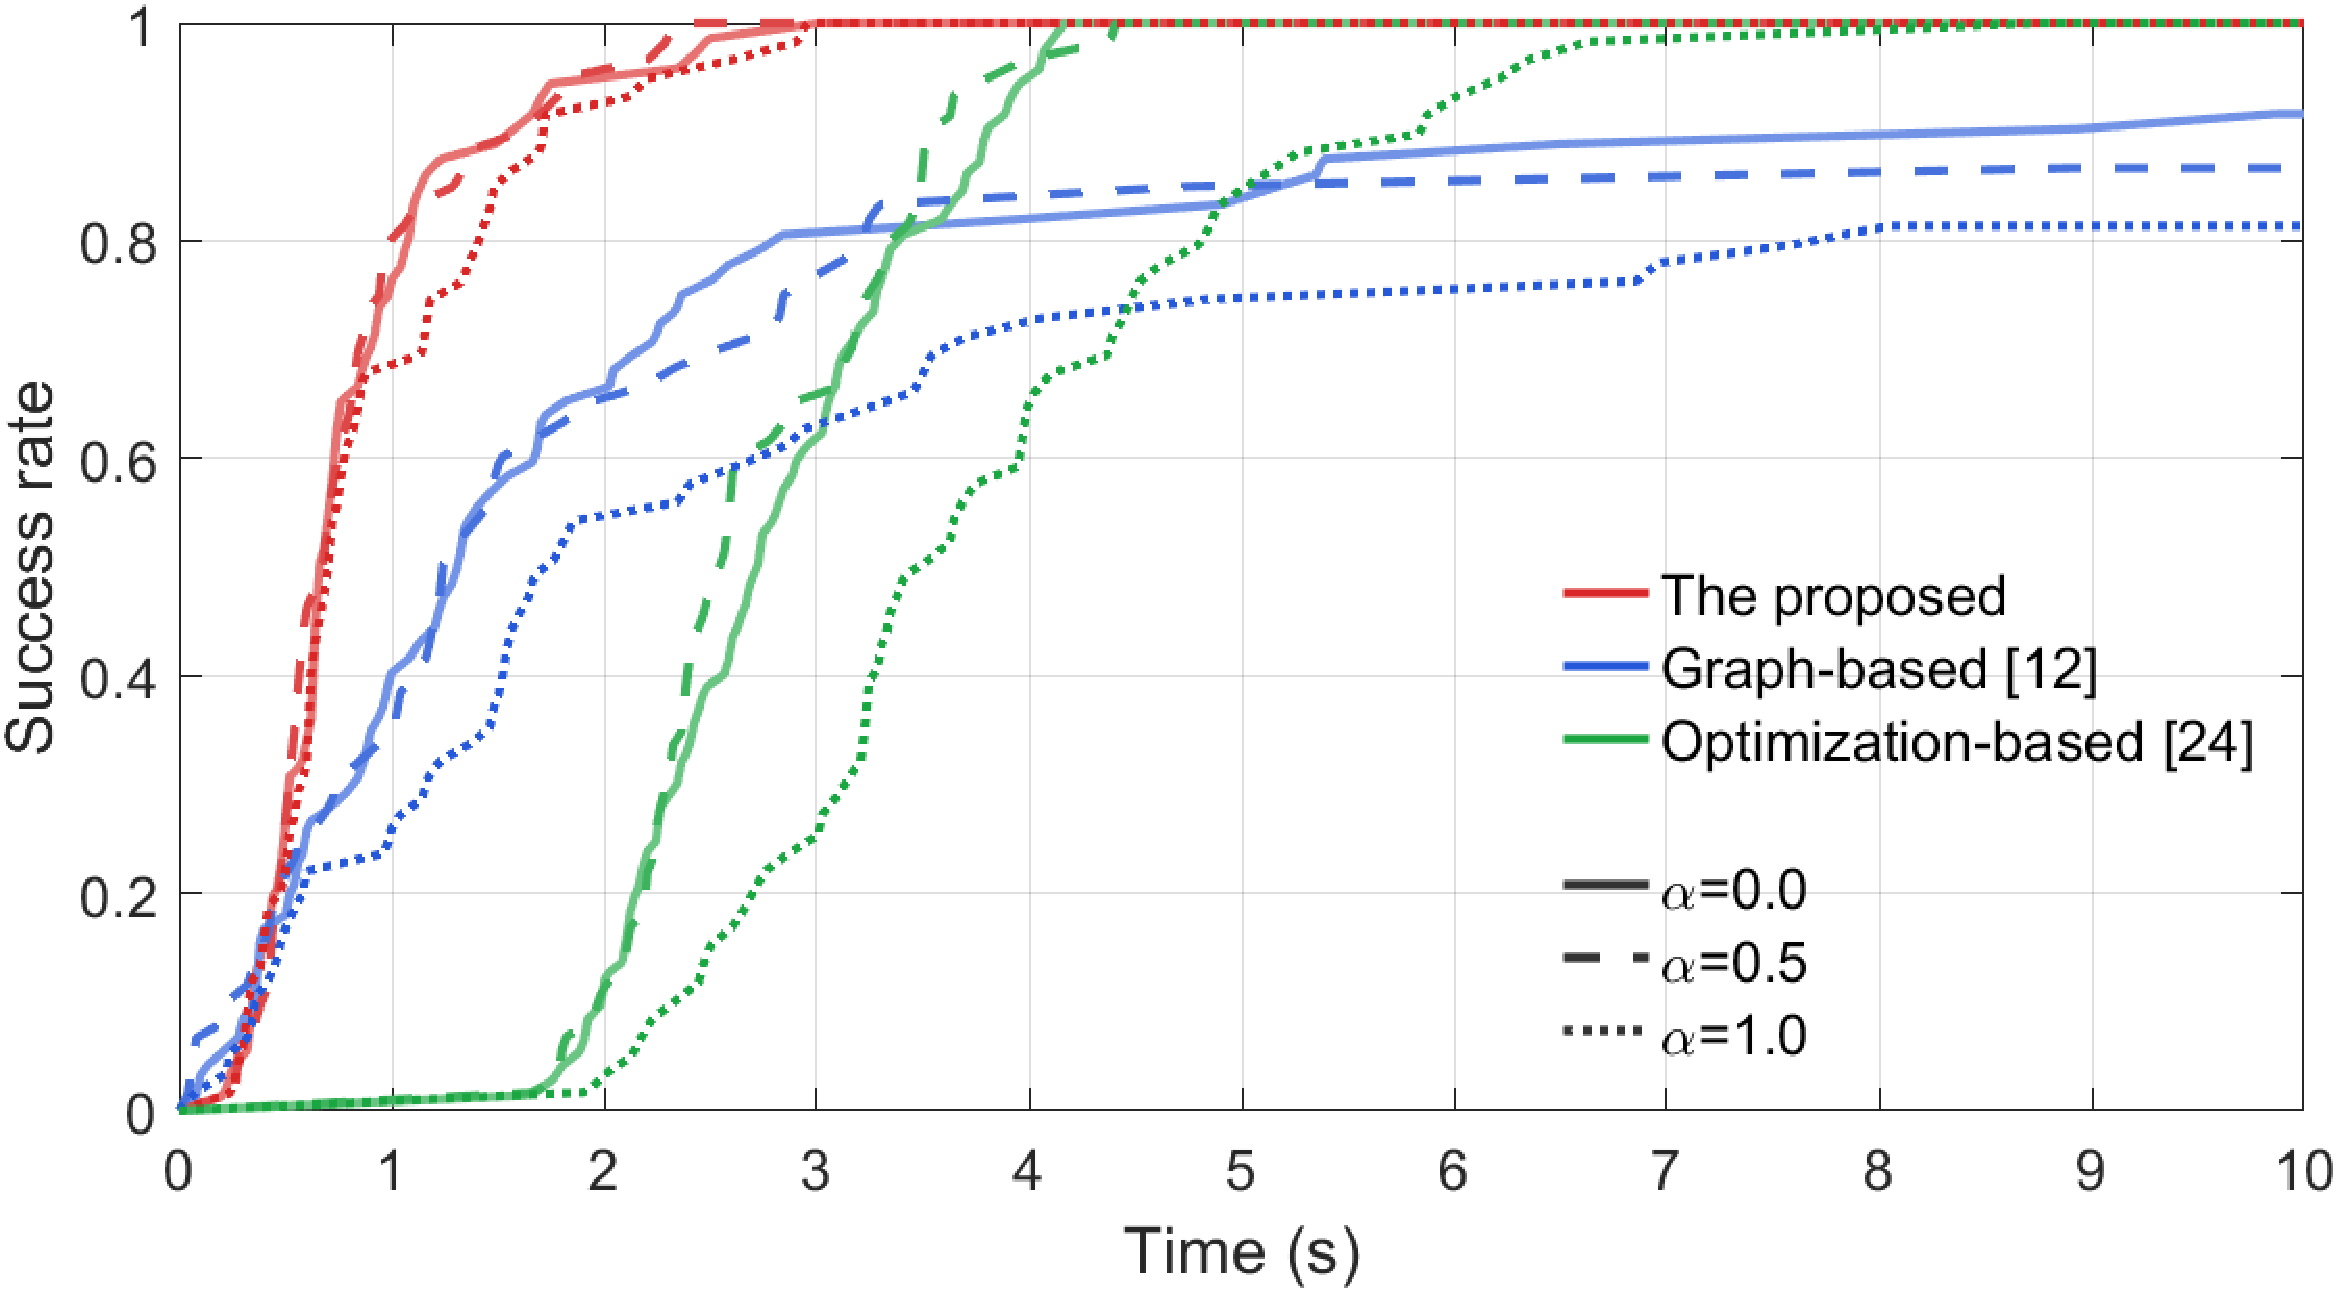
\includegraphics[width=0.90\linewidth]{Fig/verification.pdf}
    \vspace{-3mm}
    \caption{
    Normalized success rate versus computation time on CVAE-generated terrains for $\alpha\in\{0,0.5,1\}$.
    Results are evaluated on a set of $N=100$ terrains and rate is computed over the subset of terrains solved by any planner.
    Colors denote planners and line styles denote difficulty levels.
    }
    \label{fig:verification}
    \vspace{-3mm}
\end{figure}

We generate CVAE-based terrains and evaluate all three planners on the same terrains under a fixed computation-time limit.
Because some randomly generated terrains are not solvable by any of the three planners under the imposed evaluation constraints, we exclude those cases and report the success rate only over the subset solved by at least one planner.
We run each planner on each terrain and record its computation time until it first returns a feasible footstep sequence that satisfies all constraints and reaches the goal within a fixed tolerance.
This allows us to compare both overall success and how quickly successful solutions are found.

Fig.~\ref{fig:verification} plots the normalized success rate versus computation time over the subset of terrains solved by at least one planner.
Across difficulty levels, the proposed planner achieves high success rates with shorter computation times, indicating that it can reliably find feasible solutions within practical time budgets.
As terrain difficulty increases with $\alpha$, the optimization-based baseline tends to require longer computation times to find a feasible solution, although it can approach $100\%$ success rates when given sufficient time.
In contrast, the success rate of the graph-based baseline rises quickly but saturates below $100\%$, and this tendency becomes more pronounced at higher difficulty levels, suggesting that it fails to discover feasible paths within the time budget even though other methods succeed.
Overall, the proposed method consistently attains higher success rates at short computation times across these challenging CVAE-generated stepping-stone terrains.

\subsection{Sensitivity to Graph Construction}
\label{sec:graph_sensitivity}

\begin{figure}[t]    
    \centering
    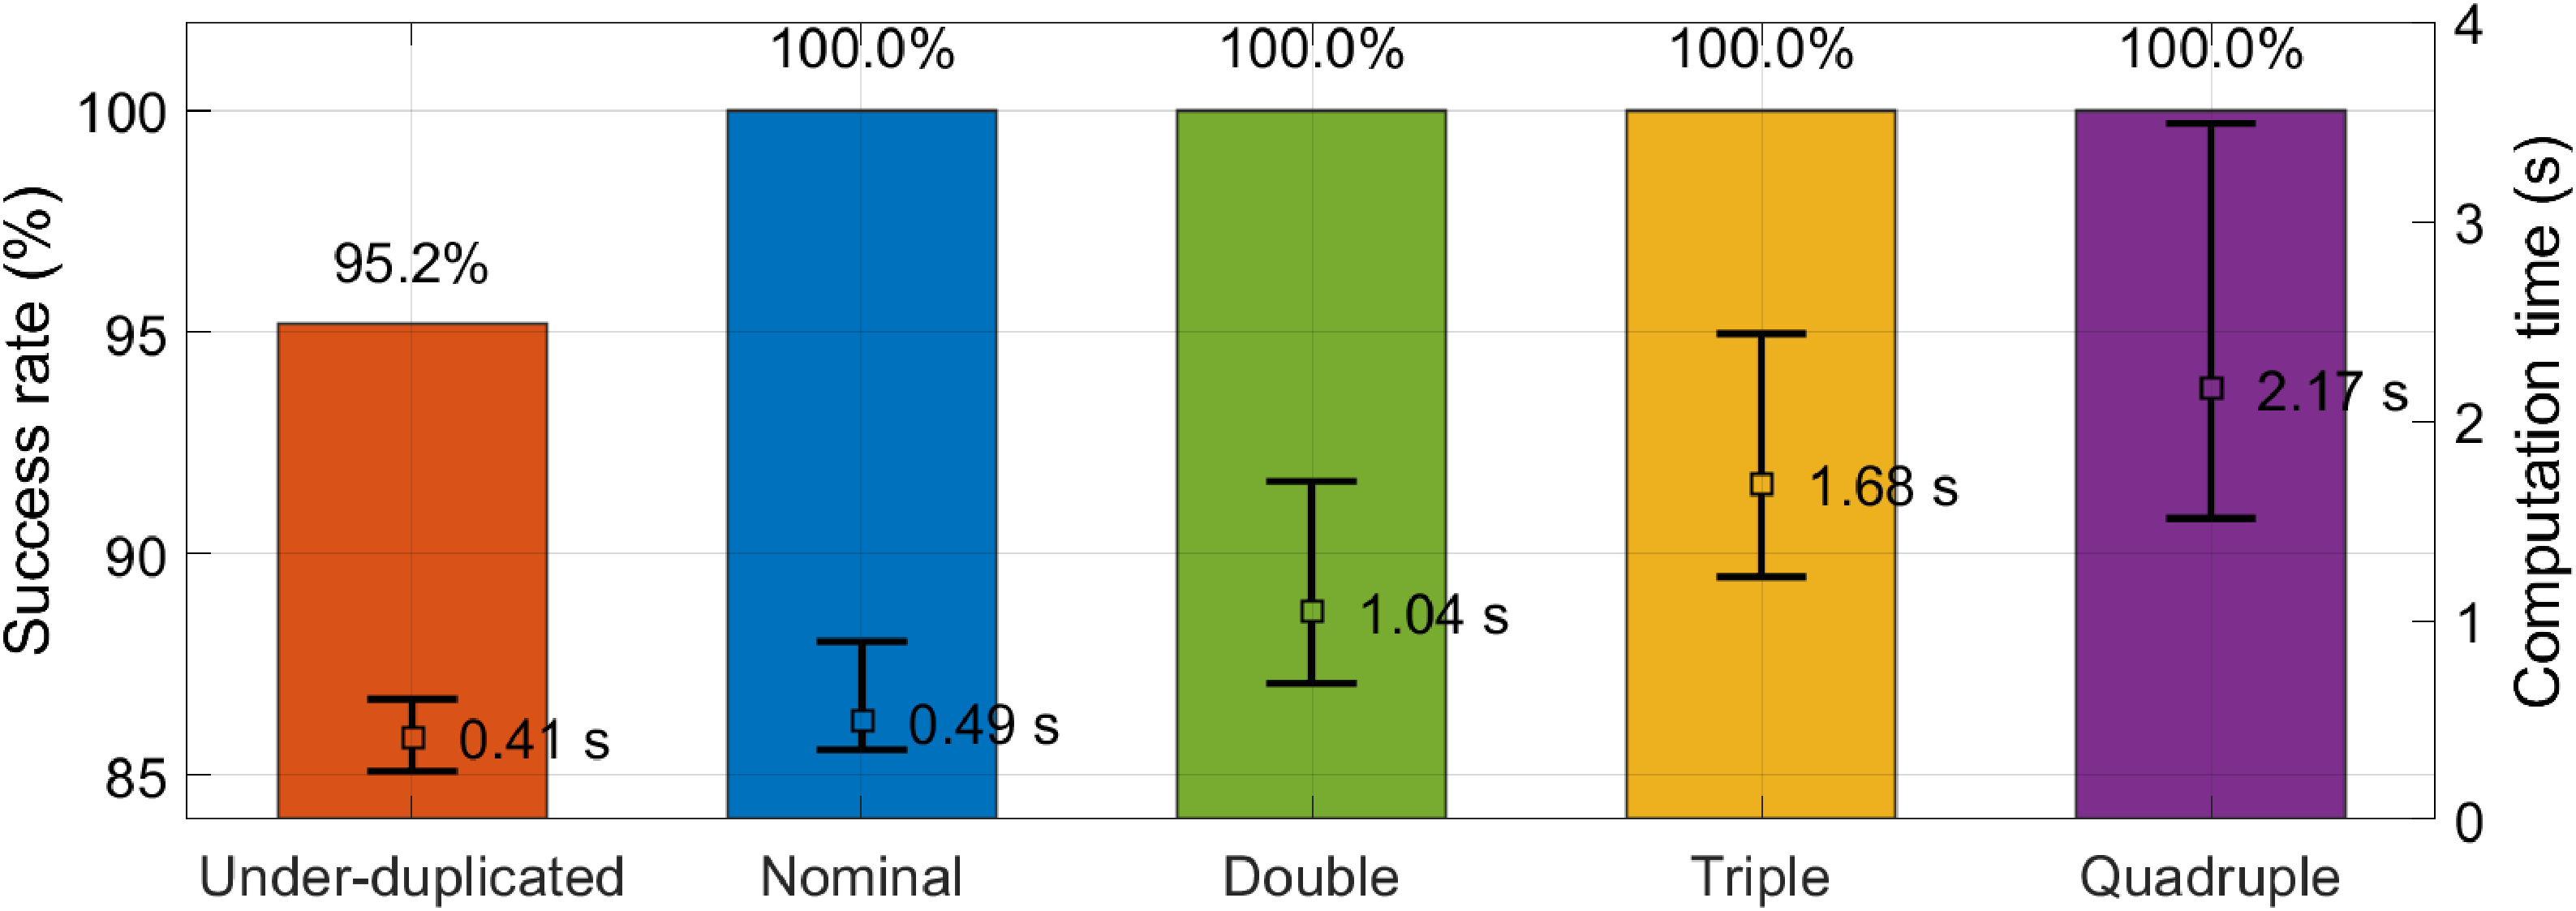
\includegraphics[width=0.95\linewidth]{Fig/figureR1.pdf}
    \vspace{-3mm}
    \caption{
    Sensitivity to vertex duplication on the CVAE-generated benchmark.
    Bars show the normalized success rate, while markers and error bars show the median computation time and its interquartile range.
    }
    \label{fig:figureR1}
    \vspace{-4mm}
\end{figure}

\begingroup
\setlength{\textfloatsep}{2pt}

\begin{table}[t]
\vspace{-4mm}
\centering
\caption{Relaxation gaps for different edge-construction rules.}
\label{tab:edge_gap_comparison}
\footnotesize
\setlength{\tabcolsep}{4pt}
\renewcommand{\arraystretch}{1.0}
\begin{tabular}{lcc}
\toprule
Statistic & Nominal sparse & Dense mode-compatible \\
\midrule
Median gap & 25.66\% & 32.66\% \\
\bottomrule
\end{tabular}
\vspace{-4mm}
\end{table}

\endgroup

We evaluate the planner's sensitivity to vertex duplication and edge construction on 100 four-region CVAE-generated terrains.
The nominal graph assigns $[5,4,4,5]$ vertices to the regions and is compared with an under-duplicated graph and graphs containing two, three, and four times as many vertices.
As shown in Fig.~\ref{fig:figureR1}, under-duplication reduces success rate by restricting representable stepping sequences, whereas further duplication maintains the 100\% success rate but substantially increases computation time.
We also compare the nominal sparse rule with a dense mode-compatible rule connecting every vertex pair permitted by the support-mode transitions.
As shown in Table~\ref{tab:edge_gap_comparison}, the dense rule increases the median relaxation gap from 25.66\% to 32.66\%, likely because additional edges introduce more fractional path alternatives and widen the gap between the relaxed and recovered costs.

\section{Real-World Deployment}

We deploy our footstep planner integrated into a full motion-planning-to-control pipeline~\cite{mesesan2025motion,schuller2026centroidal} on the torque-controlled humanoid robot, a 27-DoF robot with a height of 1.74\,m and a weight of 79.2\,kg~\cite{englsberger2014overview}.
We choose the \textit{Pump It Up} scenario, a rhythm-based arcade game, shown in Figs.~\ref{fig:main},~\ref{fig:pump_it_up}, because it couples discrete footstep sequencing with continuous foot placement under timing constraints, providing a challenging benchmark for real-time planning. 
This setting induces a receding-horizon replanning problem, where the plan must be updated at each symbol change while maintaining feasibility over upcoming steps.
We show that the proposed method is practically deployable on a humanoid platform by achieving fast replanning under strict timing constraints.

\subsection{Scenario: Pump It Up}

This paper demonstrates the \textit{Pump It Up} game as a challenging benchmark for real-time footstep planning. 
Players stand on a dance pad and step on arrow-shaped panels (e.g., $\{UR, UL, C, DR, DL\}$) when the corresponding symbols on the screen reach the top timing bar, as shown in Fig.~\ref{fig:pump_it_up}. 
This setting requires players to decide both which foot to use and where to place it, coupling discrete foot assignment with continuous foot placement.
\\
\indent
\textbf{(i) Discrete footstep sequencing.}  
Even for the same upcoming sequence of labels, multiple feasible left/right stepping strategies exist.  
Given the label window  $\{C, UR, DL, C\}$ in Fig.~\ref{fig:pump_it_up}(c), players may choose strategies such as $\{$Right--Right--Left--Left$\}$ or $\{$Left--Right--Left--Right$\}$, each representing a different discrete footstep assignment.
\\
\indent
\textbf{(ii) Continuous foot placement.}  
In addition to deciding the left--right assignment, the planner must determine the precise pose and yaw of the foot within each selected panel. 

\begin{figure}[t]
    \centering
    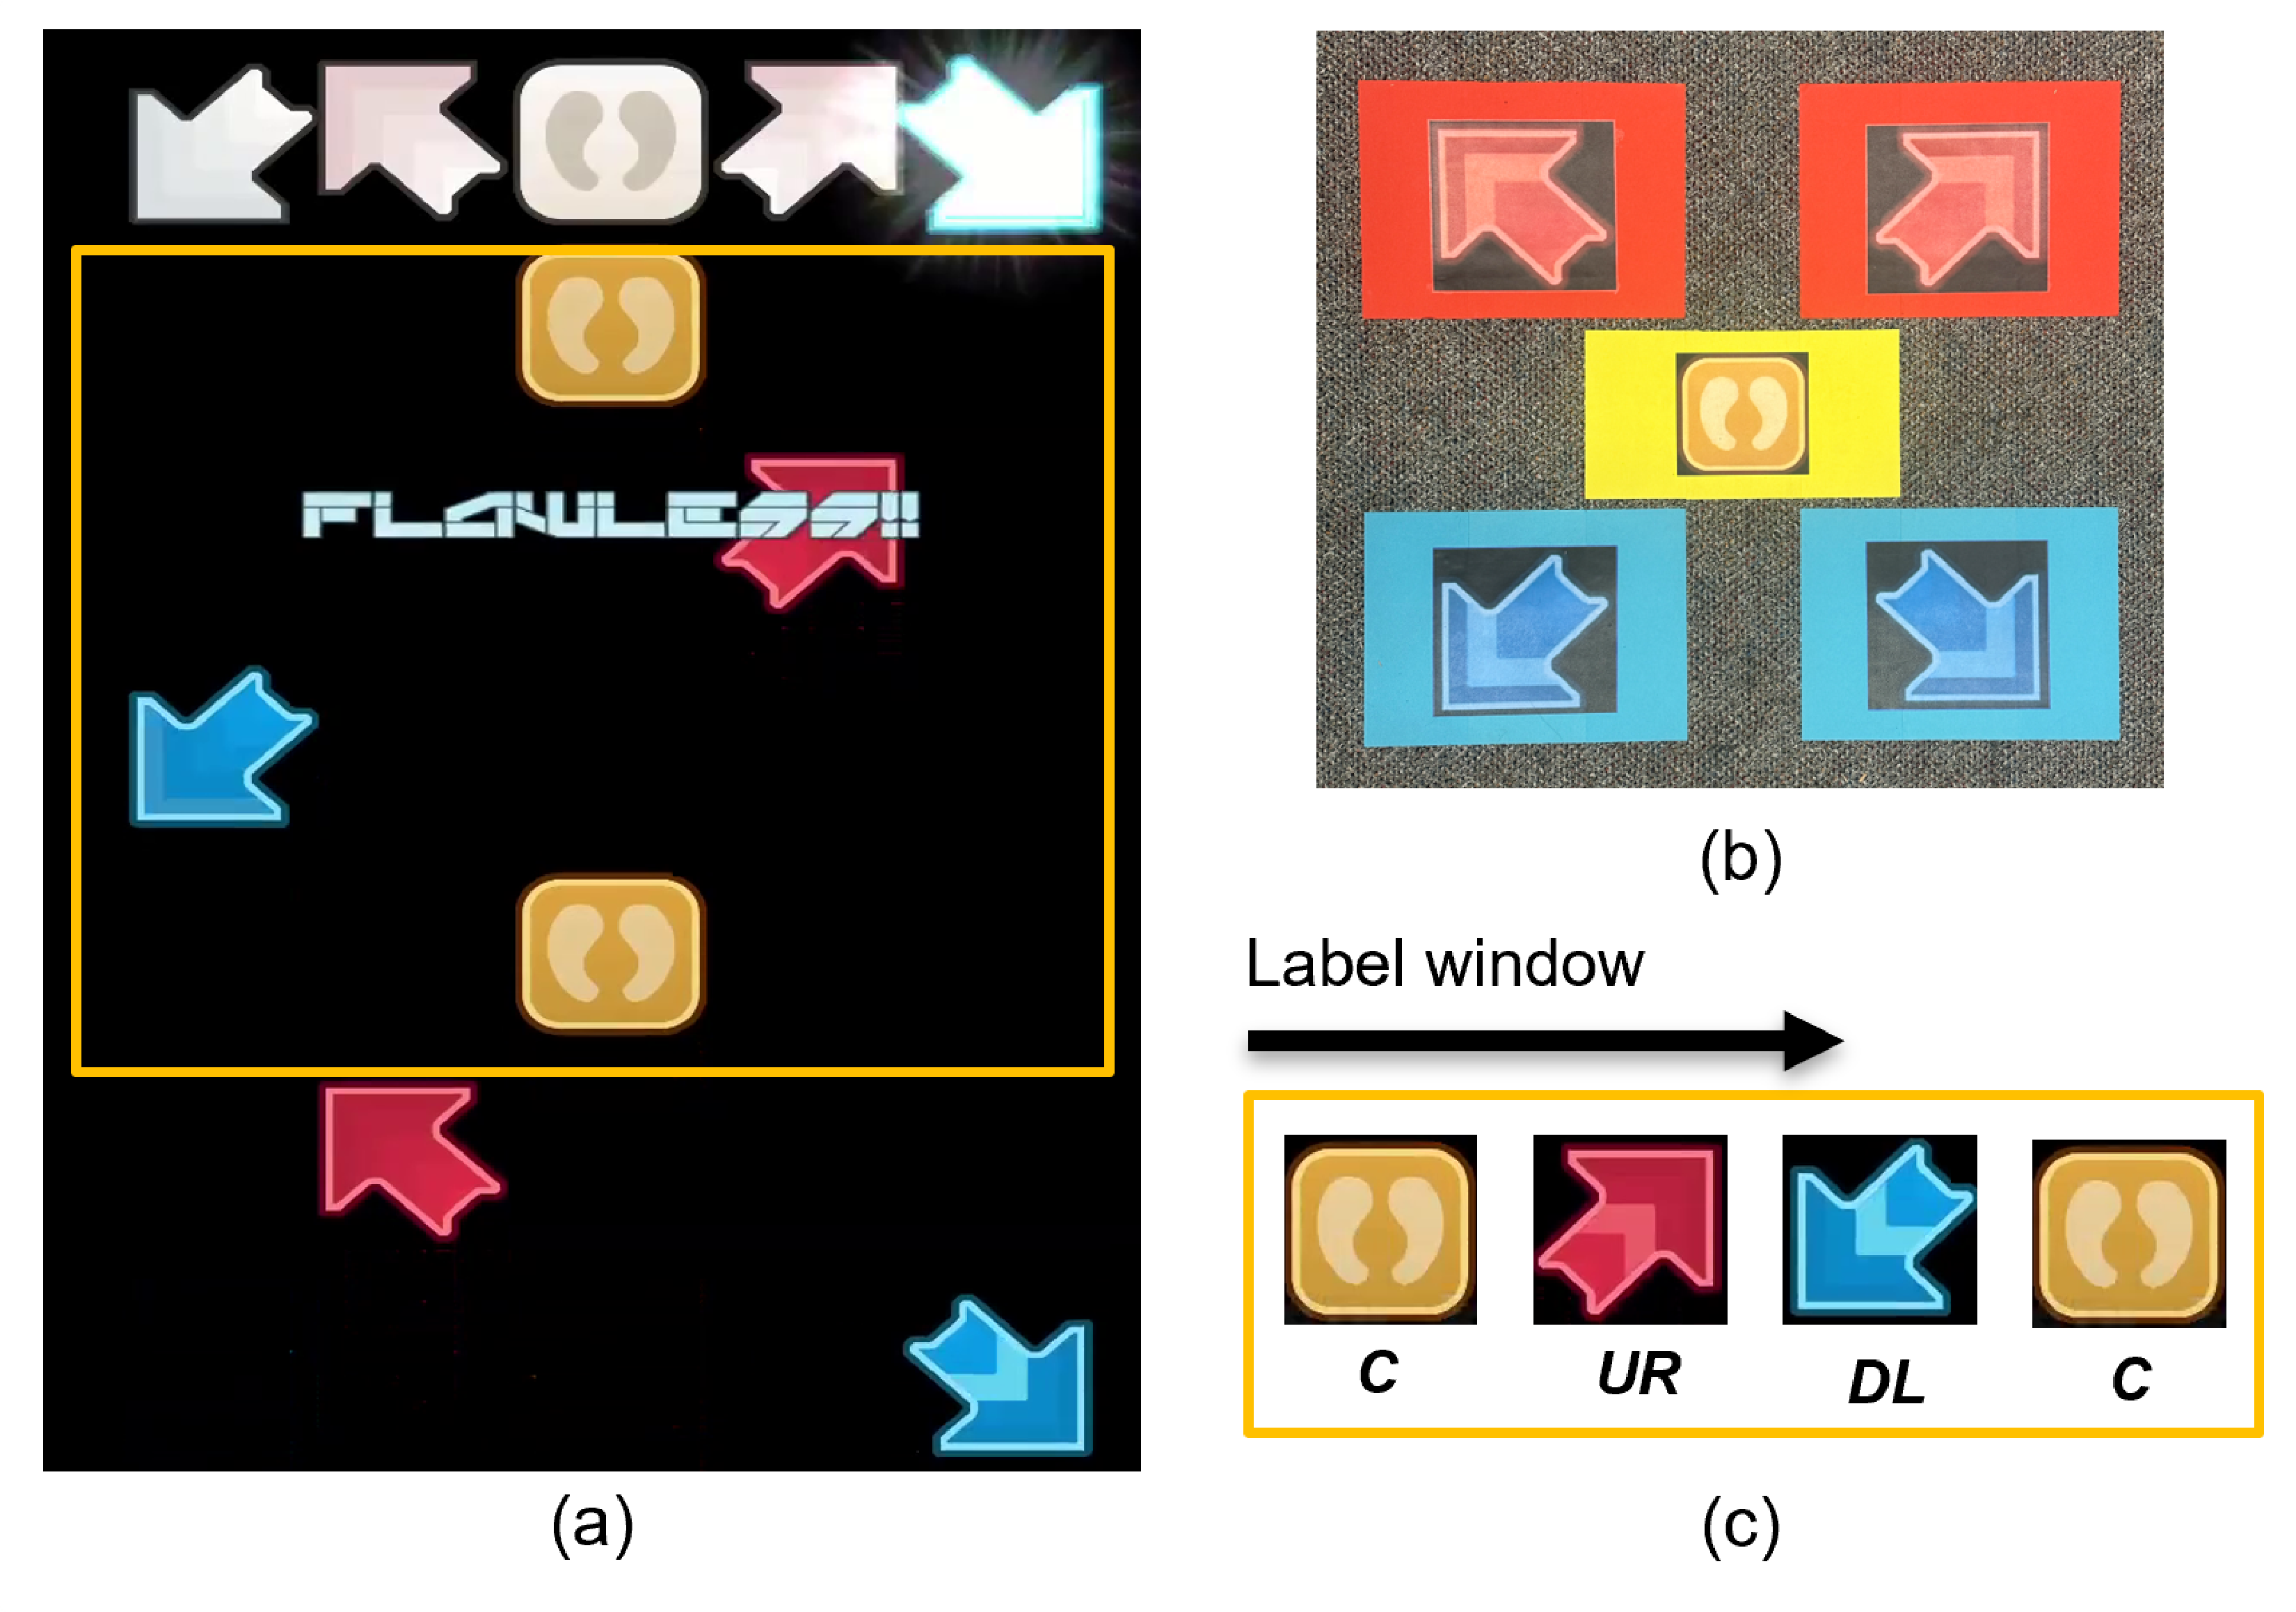
\includegraphics[width=0.70\linewidth]{Fig/pump_it_up.pdf}
    \vspace{-3mm}
    \caption{
    Illustration of the \textit{Pump It Up} game.
    (a) The game screen, where arrow symbols scroll upward and are activated by stepping on the corresponding panel as they reach the top timing bar.
    (b) The dance pad, where any point within the corresponding panel serves as a valid activation region.
    (c) The label window shows the upcoming sequence of arrow symbols to be activated in order. The window($W=4$) corresponds to the yellow boxed region in (a).
    }
    \label{fig:pump_it_up}
    \vspace{-3mm}
\end{figure} 

\subsection{Implementation Details}

The footstep plan is determined from the current pose and the upcoming label sequence within the label window.
When a new symbol is appended, the entire window must be replanned, since the new label can change the optimal intermediate steps, including both discrete foot assignments and continuous foot placements.
As the symbols scroll toward the timing bar, this replanning must be completed within each symbol-to-symbol interval so that the planner can update the plan online and maintain the best solution at each instant.
Our footstep planner is implemented using the MOSEK \cite{mosek} solver and executed on a desktop with an Intel Core i7-10700K CPU and 32 GB RAM. 
We use a six-step label window ($W=6$), matching the six upcoming symbols displayed on the game interface.
Whenever a new symbol appears at the bottom of the screen, it is appended to the end of the window while the first symbol, corresponding to the executed step, is removed, yielding the updated window for the next replanning cycle.
\begin{figure}[t]
    \centering
    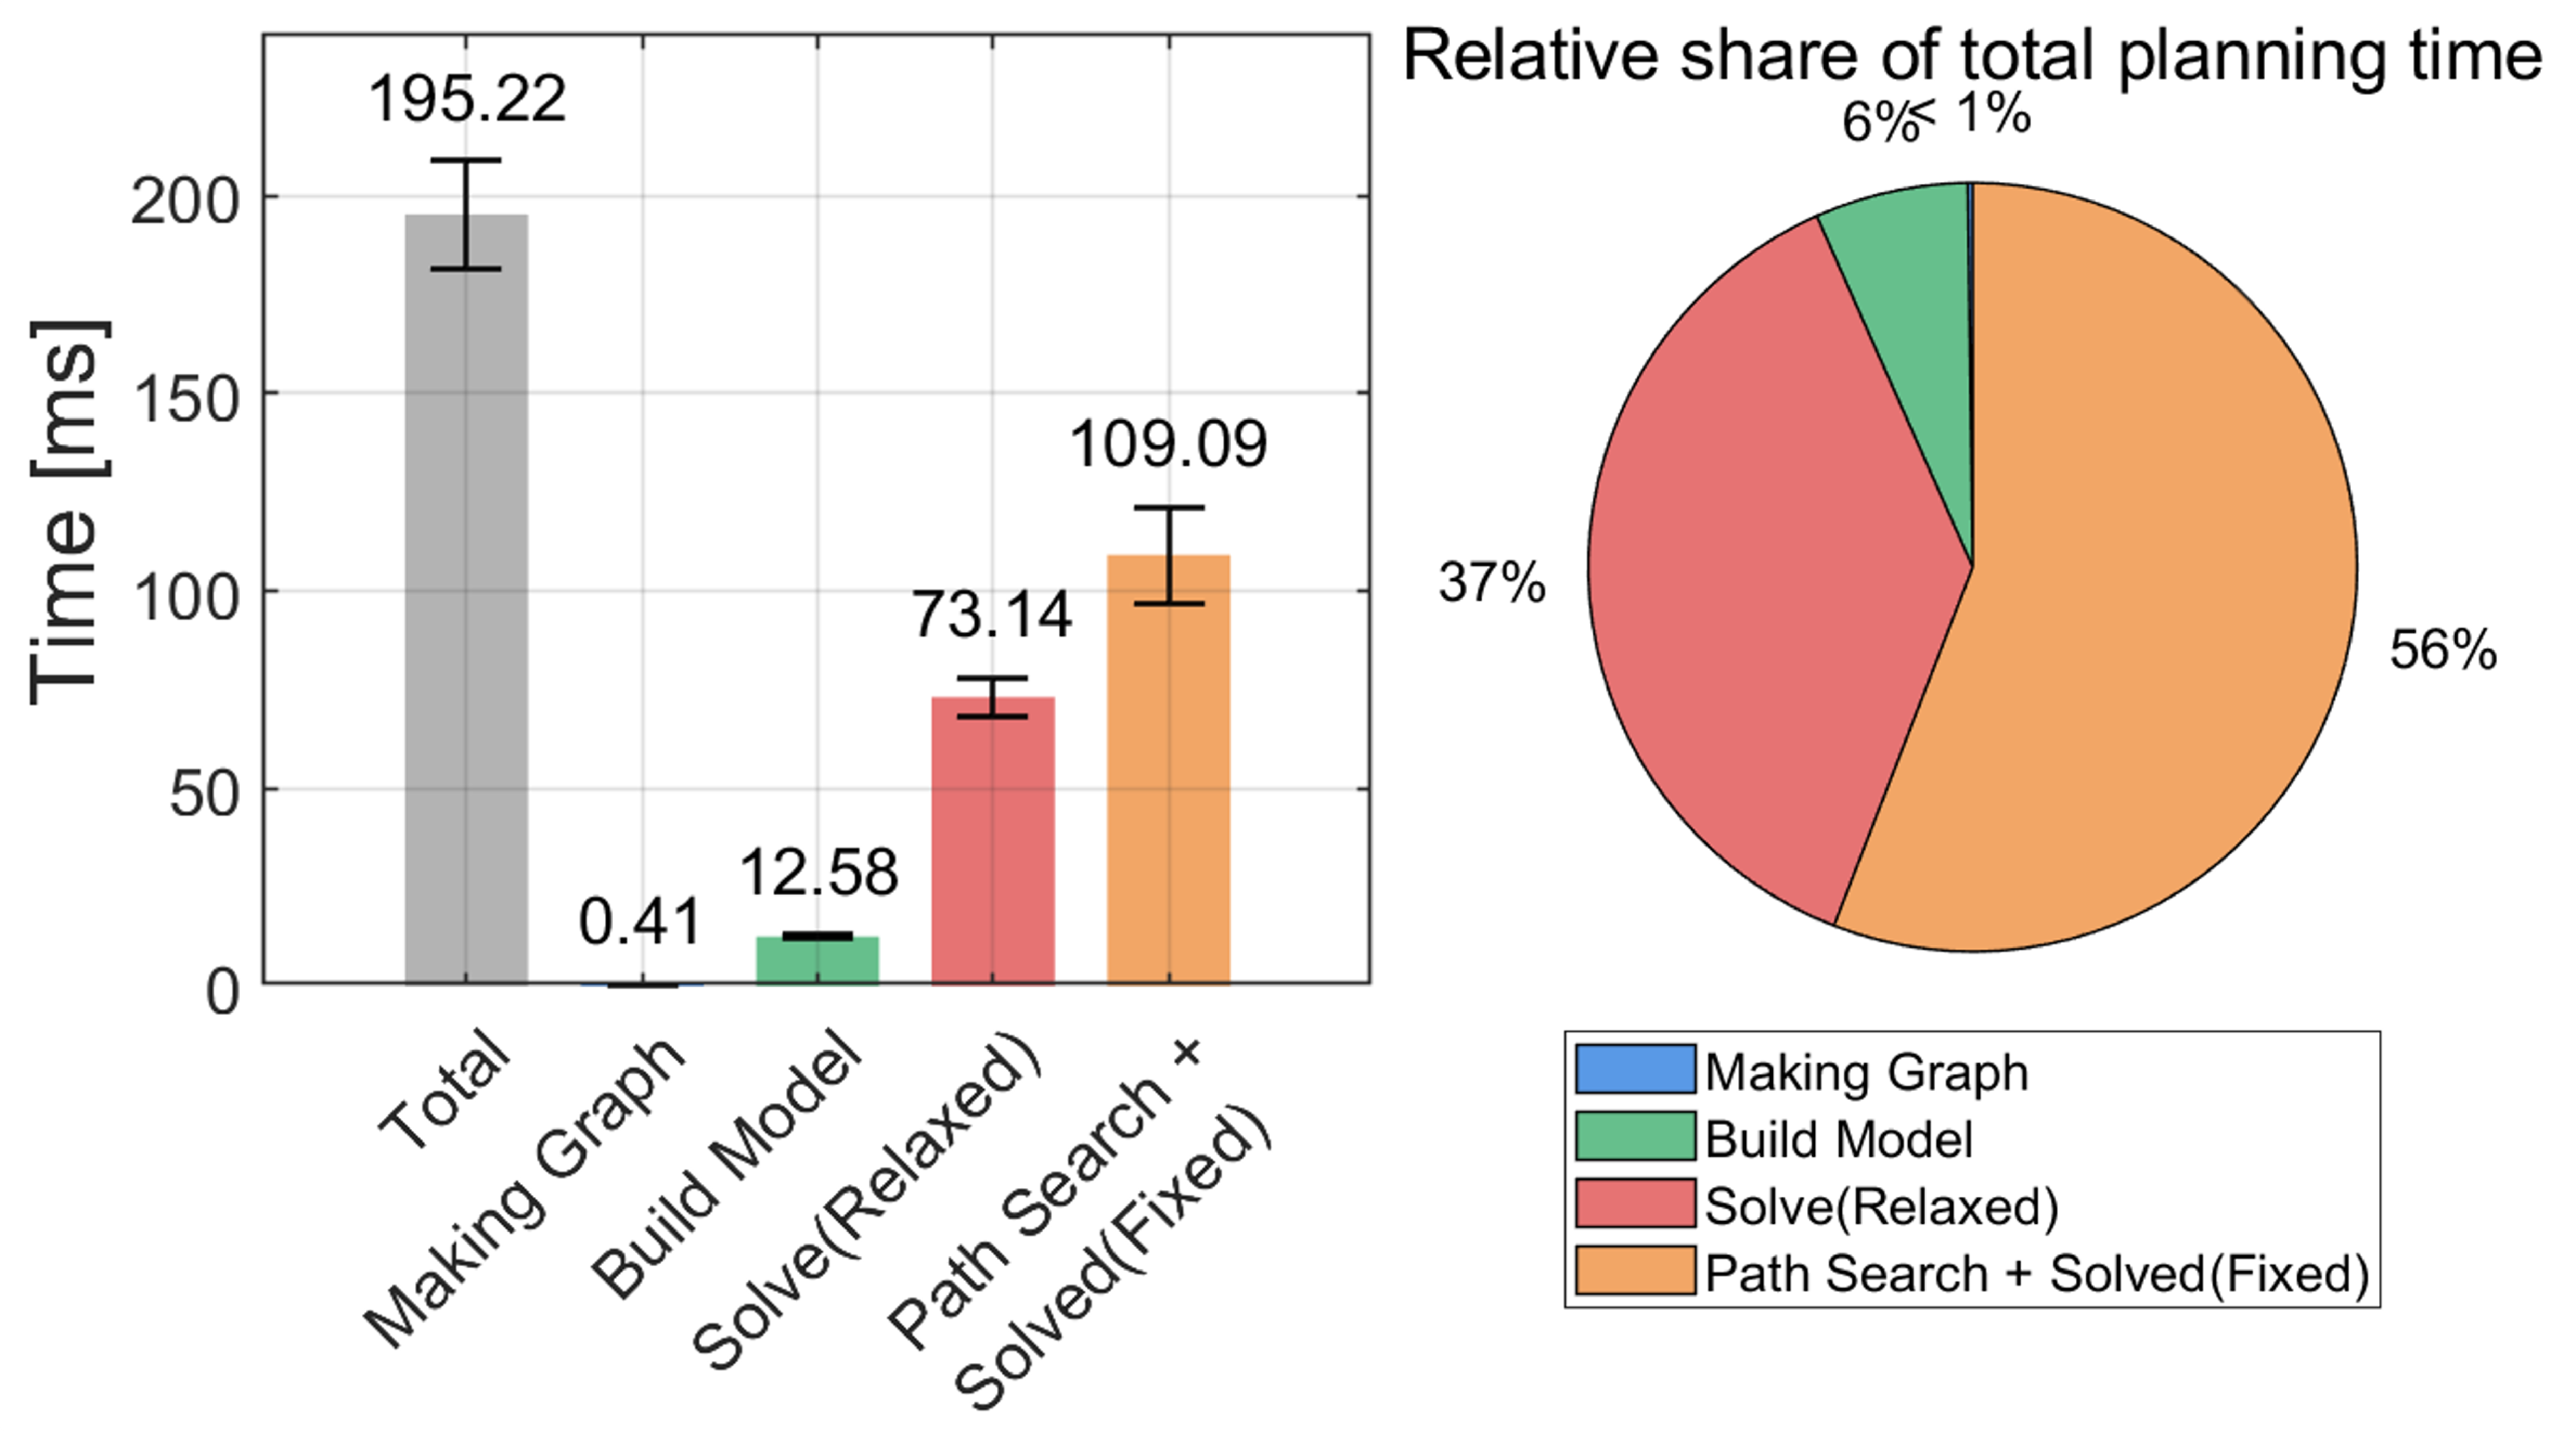
\includegraphics[width=0.95\linewidth]{Fig/data_result.pdf}
    \vspace{-3mm}
    \caption{
    Timing breakdown for each component of the planning pipeline (left), and the relative computation time (right) during the deployment.
    }
    \label{fig:data_result}
    \vspace{-3mm}
\end{figure}
\begin{figure}[t]
    \centering
    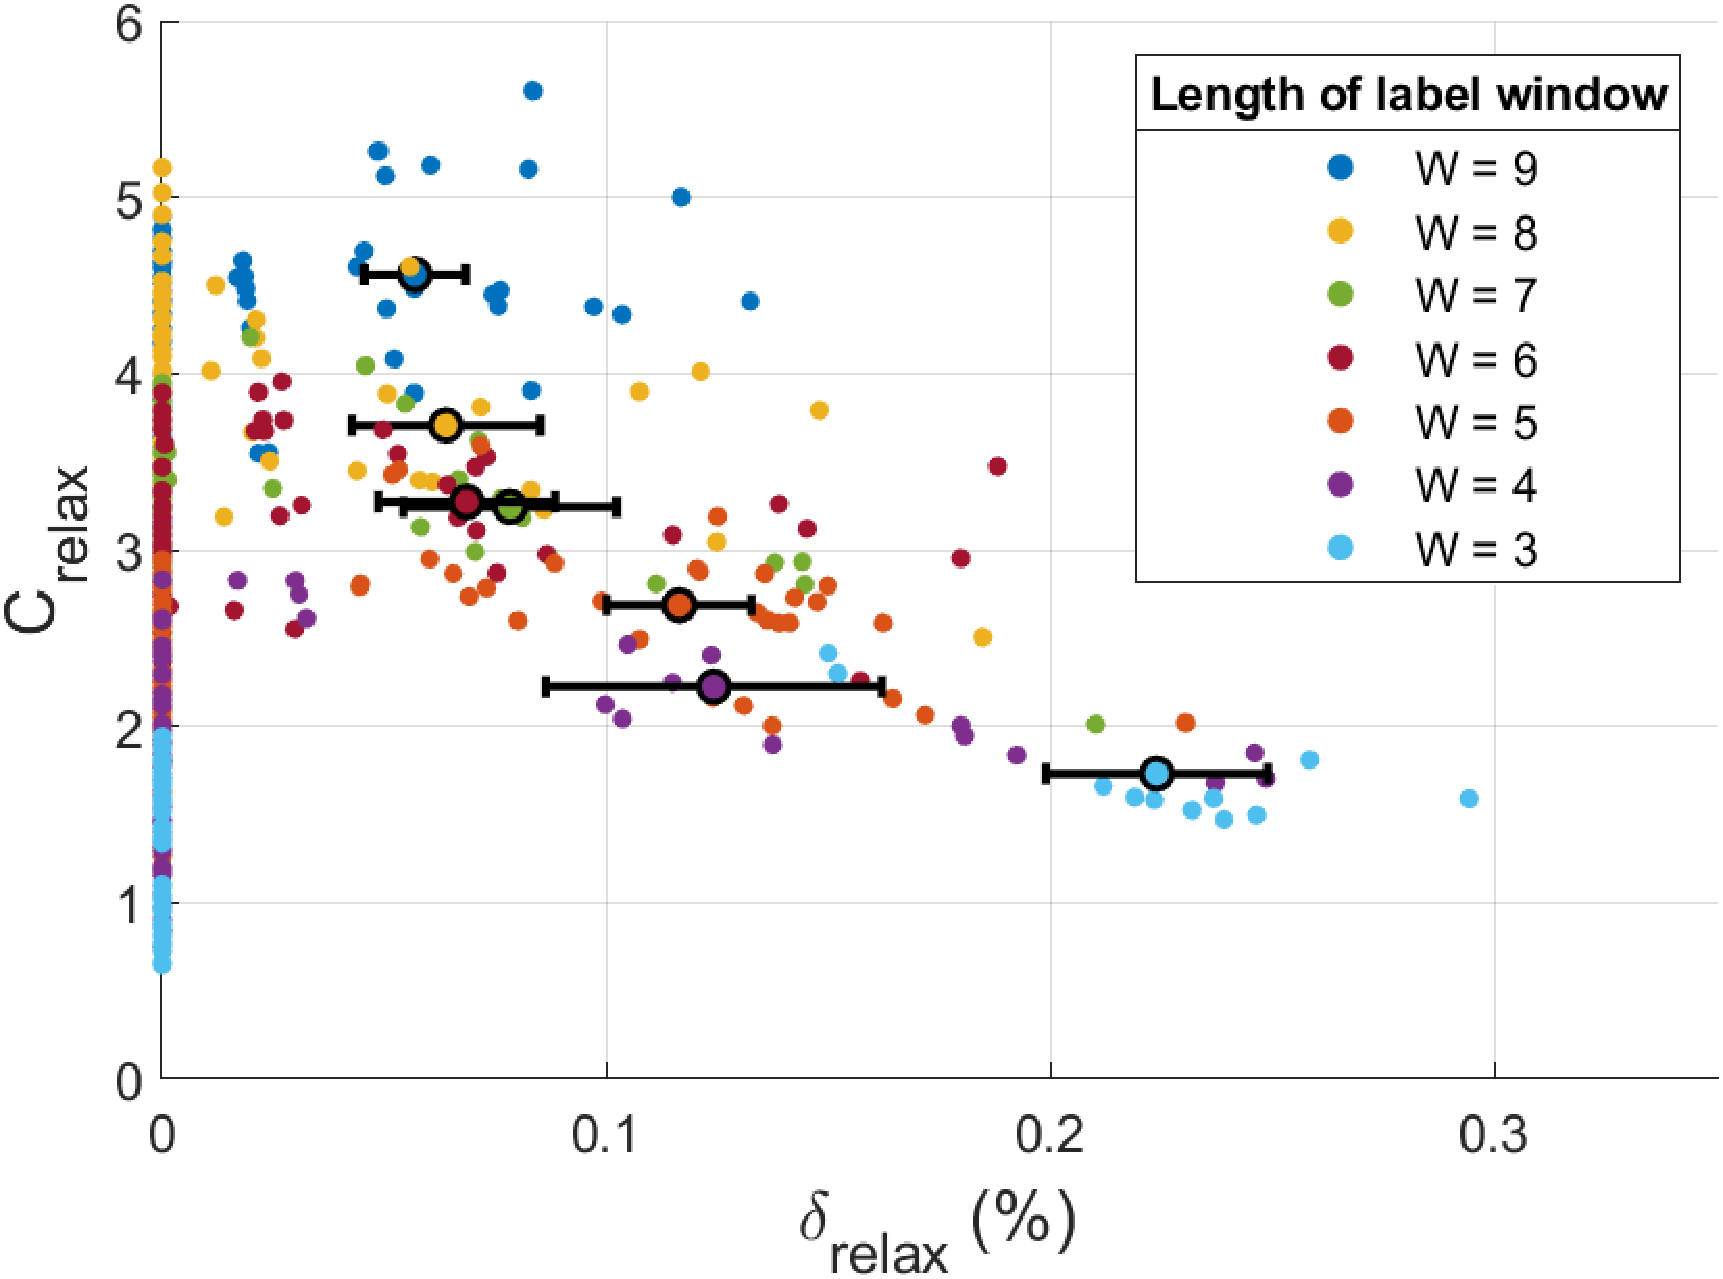
\includegraphics[width=0.75\linewidth]{Fig/Result_relaxationgap.pdf}
    \vspace{-3mm}
    \caption{Relaxed cost $C_{\mathrm{relax}}$ versus relaxation gap $\delta_{\mathrm{relax}}$ for label window lengths $W=3$--$9$ (100 replanning trials per $W$). For nonzero relaxation gaps, the mean and standard deviation for each $W$ are additionally shown.} 
    \label{fig:relax_gap}
    \vspace{-4mm}
\end{figure}
\subsection{Planner Performance}
At each planning cycle, the planner executes four stages: (i) graph construction, (ii) optimization model formulation, (iii) solving the R-MICP, and (iv) path selection followed by a fixed-path convex solve.
To evaluate runtime, we measure the duration of each stage over planning cycles during real-world deployment, as shown in Fig.~\ref{fig:data_result}.
Since the terrain is fixed in our deployment, graph construction time is small, while most computation is spent in stages (iii) and (iv).
Stage (iv) includes repeated path sampling from the relaxed edge values and fixed-path convex solves until a feasible solution is obtained.
Across repeated cycles, the proposed planner's average planning time remained below 200\,ms, well within the symbol-to-symbol interval imposed by the game rhythm.
By comparison, an offline replay showed that the proposed planner achieved 100\% on-time success by 0.3\,s, the graph-based baseline achieved 79.6\% overall feasibility, and the optimization-based baseline achieved 100\% only at 2.0\,s.
\\
\indent
We evaluate solution quality by examining relaxation tightness.
Following \eqref{eq:relax_gap_def}, Fig.~\ref{fig:relax_gap} plots the relaxation gap $\delta_{\mathrm{relax}}$ versus the relaxed cost $C_{\mathrm{relax}}$.
Because $C_{\mathrm{relax}}$ provides a lower bound on the original MICP, $\delta_{\mathrm{relax}}$ upper-bounds the optimality gap of the rounded solution and serves as a quantitative measure of solution quality.
The relaxation gap remains below $0.3\%$ for all tested window lengths ($W=3$--$9$).
Among the nonzero-gap instances, the average relaxation gap tends to decrease with the window length, likely because larger windows add downstream constraints that reduce ambiguity in the discrete decisions.
Larger gaps mainly occur for short windows and low $C_{\mathrm{relax}}$, where near-equivalent choices coexist.


\section{Conclusion}

In this work, we presented a GCS-based footstep planner that jointly optimizes the discrete stepping sequence and continuous foot placements within a unified framework.
We leveraged a tight SDP relaxation and an efficient rounding-and-fixing pipeline to compute high-quality solutions under real-time planning budgets.
The proposed planner was validated through real-world deployment on the humanoid robot under strict timing constraints, demonstrating robust and repeatable performance in the \textit{Pump It Up} scenario.
Despite these results, the SDP relaxation can become looser in more complex settings or cases requiring large rotations, while solution quality and runtime remain sensitive to graph construction.
It assumes that candidate convex foothold regions and their associated graph representation are available. 
Moreover, our footstep planner does not explicitly model step timing or robot dynamics. 
In future work, we will improve relaxation tightness in challenging cases, develop perception-driven graph construction strategies that generalize across diverse and unstructured terrains, and extend the formulation to incorporate timing and dynamic constraints for more agile real-world locomotion.


%\section*{Acknowledgments}
%This should be a simple paragraph before the References to thank those individuals and institutions who have supported your work on this article.



%{\appendix[Proof of the Zonklar Equations]
%Use $\backslash${\tt{appendix}} if you have a single appendix:
%Do not use $\backslash${\tt{section}} anymore after %$\backslash${\tt{appendix}}, only $\backslash${\tt{section*}}.
%If you have multiple appendixes use $\backslash${\tt{appendices}} then %use $\backslash${\tt{section}} to start each appendix.
%You must declare a $\backslash${\tt{section}} before using any %$\backslash${\tt{subsection}} or using $\backslash${\tt{label}} 
%($\backslash${\tt{appendices}} by itself
% starts a section numbered zero.)}



%{\appendices
%\section*{Proof of the First Zonklar Equation}
%Appendix one text goes here.
% You can choose not to have a title for an appendix if you want by leaving the argument blank
%\section*{Proof of the Second Zonklar Equation}
%Appendix two text goes here.}



\bibliography{ref}
\bibliographystyle{IEEEtran}


%\newpage

 
%\vspace{11pt}

%\bf{If you include a photo:}\vspace{-33pt}
%\begin{IEEEbiography}[{\includegraphics[width=1in,height=1.25in,clip,keepaspectratio]{fig1}}]{Michael Shell}
%Use $\backslash${\tt{begin\{IEEEbiography\}}} and then for the 1st argument use $\backslash${\tt{includegraphics}} to declare and link the author photo.
%Use the author name as the 3rd argument followed by the biography text.
%\end{IEEEbiography}

%\vspace{11pt}

%\bf{If you will not include a photo:}\vspace{-33pt}
%\begin{IEEEbiographynophoto}{John Doe}
%Use $\backslash${\tt{begin\{IEEEbiographynophoto\}}} and the author name as the argument followed by the biography text.
%\end{IEEEbiographynophoto}




%\vfill

\end{document}


